\documentclass[14pt]{article}
\usepackage[english]{babel}
\usepackage{amsmath, amsthm, amssymb, graphicx, xcolor, mathtools, tikz, booktabs, natbib, setspace, etoolbox, needspace, xcolor, multirow, enumerate }
\usepackage[bf, tiny, center]{titlesec}
\usepackage[footnotesize, bf]{caption}
\usepackage[font+=footnotesize, labelfont=bf]{subcaption}
\usepackage[margin=1.5in]{geometry}
\usepackage{titling}
\usepackage{blindtext}
\usepackage{tikz}
\usepackage{pifont}



%environments
\theoremstyle{plain}
\newtheorem{thm}{Theorem}[section]
\newtheorem{cor}[thm]{Corollary}
\newtheorem{lemma}[thm]{Lemma}
\newtheorem{prop}[thm]{Proposition}

\theoremstyle{definition}
\newtheorem{defn}{Definition}[section]
\newtheorem{ass}{Assumption}
\newtheorem{example}{Example}
\newtheorem{obs}{Observation}
\newtheorem{property}{Property}
\newtheorem{condition}{Condition}
\newtheorem{claim}{Claim}
\newtheorem{explanation}{Explanation}
\setlength{\parindent}{0.5cm}
\theoremstyle{remark}
\newtheorem{rem}{Remark}[section]
\newtheorem{conjecture}[thm]{\textbf{Conjecture}}


%\newcommand{\clrblue}[1]{{\color{blue!60!green} #1}}
\definecolor{manganese}{rgb}{0, 0.4, 0.6}
\newcommand{\clrblue}[1]{{\color{manganese} #1}}
\newcommand{\note}[1]{{\footnotesize \color{manganese} [#1]}}
\newcommand\given[1][]{\:#1\vert\:}
%multiline comments
\newcommand{\comment}[1]{}
\newcommand{\n}{$\text{ }$}
\newcommand{\clrred}[1]{{\color{red} #1}}



%measure theory
\newcommand{\set}[1]{\left\lbrace #1 \right\rbrace}
\newcommand{\bset}[1]{\bigl\{ #1 \bigr\}}
\newcommand{\where}{\ \middle\vert\;}
\newcommand{\bwhere}{\ \big\vert\;}
\newcommand{\abs}[1]{\left\vert #1 \right\vert}
\newcommand{\norm}[2][]{{\left\Vert #2 \right\Vert}_{#1}}
\newcommand{\bnorm}[2][]{\bigl\Vert #2 \bigr\Vert_{#1}}
\DeclareMathOperator*{\argmax}{arg\,max}
\DeclareMathOperator*{\argmin}{arg\,min}
%analysis
\newcommand{\tr}[1]{#1^{\top}}
\newcommand{\xmatrix}[1]{\!\left(\:\begin{matrix} #1 \end{matrix}\:\right)\!}
\newcommand{\funcdef}[1]{\left\lbrace \hspace{-1.2mm}
	\setlength{\arraycolsep}{3mm} \begin{array}{ll} #1 \end{array}
	\setlength{\arraycolsep}{0mm} \hspace{-1.8mm} \right.
}

%indicator function
\newcommand{\one}{1}
\newcommand{\indicator}[1]{\one_{\left\lbrace #1\right\rbrace}}
\DeclareRobustCommand\1{\futurelet\oneNext\oneCheck}
\def\oneCheck{%
	\ifx\bgroup\oneNext \expandafter\indicator%
	\else%
	\expandafter\one%
	\fi%
}

%probability theory
\newcommand{\E}[2][]{\mathbb{E}_{#1}\left[#2\right]}
\newcommand\givenbase[1][]{\:#1\lvert\:}
\renewcommand{\S}{\mathcal{S}}
\renewcommand{\H}{\mathcal{H}}
\newcommand{\R}{\mathbb{R}}





\title{Search for niches or generics? \\Product designs with heterogeneous search costs}
\author{AU Pak Hung, HSU Ke Cheng}
\date{July 21, 2024}
\graphicspath{{../}{./}}
\begin{document}
\begin{titlingpage}
    \maketitle
    \begin{abstract}
           Building on Wolinsky's (1986) sequential search model with differentiated products, this paper introduces search cost heterogeneity to analyze how firms leverage observable product designs to influence consumer search behavior. In equilibrium, consumers’ search patterns form a partitioned structure: those with low search costs tend to seek niche products, while consumers facing higher search costs gravitate toward standardized products. In the case of two product designs, a reduction in search costs may lead to higher prices for both if the endogenous shift in consumer search modes—the composition effect—dominates the search-encouraging effect. Additionally, we demonstrate that prices respond asymmetrically to decreases in search costs based on the relative position within the distribution where the shock occurs. Specifically, improvements in search technology benefiting consumers with initially low search costs tend to have anti-competitive effects, whereas those benefiting higher-cost searchers can be pro-competitive. 
    \end{abstract}
\end{titlingpage}
\section{Introduction}
Improvements in search technology have shifted aggregate consumption toward specialty products, a pattern known as the long-tail effect (Brynjolfsson et al., 2006; Anderson, 2006). As Anderson (2006) observes, the Pareto principle has increasingly given way to a ``98 percent rule,'' under which nearly every available product finds buyers. In his words, ``Apple said that every one of the 1 million tracks in iTunes had sold at least once... Netflix reckoned that 95 percent of its 25,000 DVDs are rented at least once a quarter.'' This negative relationship between search friction and sales concentration arises from the interaction between demand and supply. On the demand side, better search tools enable consumers to explore, evaluate, and purchase specialized products that would otherwise be difficult to find. On the supply side, anticipating this expanded demand for niches, firms find it worthwhile to offer products tailored to narrower tastes, which broadens the assortment available in the market. Controlling for these supply-side changes in product assortment, Brynjolfsson et al.\ (2011) show that sales remain less concentrated when search costs fall, indicating that lower search costs also directly shift consumers' search behavior toward niche products.

This paper models that demand channel and asks whether the negative relationship between search costs and product nicheness holds at the individual level, that is, whether consumers with lower search costs search for niche products while consumers with higher search costs search for generic products. We then study how improvements in search technology affect consumers' choices between niches and generics and the resulting equilibrium prices. In our model, ex-ante identical firms choose product designs ranked in dispersive order, and consumers differ in their search costs. A generic design induces a concentrated match-value distribution, whereas a niche design induces a dispersed distribution with a fatter right tail. Product designs are observable before search begins, so firms can use design choices to affect consumers' search decisions, and consumers can choose which design segment to search rather than sampling randomly across the entire market. This observability is natural in practice. Before entering Starbucks to try a seasonal release such as a salted caramel latte, a customer knows she will get something familiar and broadly acceptable, even if it is not her favorite. By contrast, a buyer visiting a specialty coffee shop for Kopi Luwak knows she may encounter a polarizing flavor that is either a great match or a poor one. On an e-commerce platform, shoppers looking for mainstream products can sort listings by sales volume before reading item descriptions, while shoppers looking for niche products can filter by a specific feature.

Because consumers' search strategies depend on firms' design and pricing choices while firms' design choices depend on how consumers with different search costs sort across segments, the two sides of the market are closely intertwined. Even so, the model delivers a clean equilibrium characterization and sharp comparative statics. When consumers' search costs are sufficiently varied, multiple product designs arise endogenously in equilibrium, and firms offering more niche designs charge higher prices. Consumers' search strategies take a monotone partitional form. Consumers in the lowest search-cost interval search the most niche segment, those in the next lowest interval search the next niche segment, and consumers with higher search costs search progressively broader segments. Intuitively, low-search-cost consumers can afford to be picky and keep searching until they find a high match value, so they are drawn to the thicker right tail of a niche design, whereas high-search-cost consumers mainly want to avoid a poor match and prefer the concentrated distribution of a standardized product. To test this prediction, we use more than ten million user-item observations from Alibaba's Tianchi platform. Using a shopper's total number of clicks as an inverse proxy for search cost and an item's total clicks across all users as a measure of popularity, we find that more active searchers tend to click on less mainstream items, consistent with our partitional sorting result.

In our comparative statics, we show that a reduction in search costs can cause firms across all product designs to raise their prices. To see why, we decompose the effect of lower search costs into an intensive margin and an extensive margin. On the intensive margin is the standard search-encouraging effect. Holding the set of shoppers in a segment fixed, lower search costs make consumers more demanding and lengthen search, which intensifies price competition and pushes prices down. On the extensive margin is a compositional effect that works in the opposite direction. At a lower search cost, the pickiest consumers in a broader segment switch to a neighboring, more niche segment. Because these switching consumers had the lowest search costs in the broad segment they leave, but have the highest search costs in the niche segment they join, the average search cost rises in both segments. Facing a customer pool with a higher average search cost, every firm, whether offering a broad or a niche design, has an incentive to raise its price. We identify sufficient conditions under which the compositional effect on the extensive margin outweighs the search-encouraging effect on the intensive margin, so that a search-cost reduction raises prices across the market.

This decomposition also explains why prices respond differently depending on whether search costs fall for low-cost or high-cost shoppers. Consider a retail market in which tech-savvy consumers browse online with low search costs, whereas less tech-savvy consumers visit brick-and-mortar stores with high search costs. Suppose search costs fall only for the low-cost group, for instance because e-commerce platforms introduce better attribute filters, price-comparison plugins, or AI search tools. Lower search costs in the niche segment make niche products more attractive and draw the lowest-cost shoppers away from the standardized segment. Standardized firms see no direct reduction in the search costs of their remaining customers, yet they lose their most price-sensitive shoppers, so the average search cost in the standardized segment rises and standardized prices go up. Niche prices can also rise if enough higher-cost shoppers switch into the niche segment. By contrast, suppose that search costs fall only for the high-cost group, for instance through clearer in-store signage, better shelf organization, or improved transit access to physical stores. Competition intensifies directly in the standardized segment and lowers standardized prices. That price drop attracts intermediate-cost shoppers away from the niche segment and into the standardized segment. Here the switching of shoppers reinforces competition in both markets. The niche segment loses its highest-cost shoppers, while the standardized segment gains shoppers who have lower search costs than its existing customers, so average search costs and equilibrium prices fall in both segments. As a result, search-cost reductions that benefit low-cost shoppers tend to be anti-competitive, whereas those that benefit high-cost shoppers are pro-competitive.

\medskip
\noindent \textbf{Literature Review}

Our paper builds on the sequential search model with differentiated products pioneered by Wolinsky (1986) and Anderson and Renault (1999). Within this framework, Bar-Isaac et al.\ (2012) and Larson (2013) endogenize product design by allowing firms to choose parameters that govern the dispersion of consumers' taste shocks.\footnote{Similar insights appear earlier in Kuksov (2004), where product design is modeled as location choice, and Cachon et al.\ (2008), where market expansion from a broader assortment offsets stronger price competition under lower search costs.} Bar-Isaac et al.\ (2012) show that equilibrium prices and profits can rise as search costs fall because firms shift endogenously from broad to niche designs, and the resulting increase in product dispersion outweighs the search-encouraging effect. Their work also accounts for the coexistence of the superstar and long-tail effects as search costs decline, since longer search durations benefit high-quality firms while intermediate-quality firms switch from broad to niche designs.

Although both papers study product design, our model differs from Bar-Isaac et al.\ (2012) in two main ways. First, product designs in our model are observable before search, allowing consumers to narrow their consideration sets and conduct design-directed search. Second, firms in our model are ex-ante symmetric rather than vertically differentiated, and consumers vary in their search costs. Firms therefore adopt different designs in equilibrium not because of ex-ante quality differences, but because they target different search-cost segments. In technical terms, a firm's price and design choices depend on the position of its marginal consumers in the valuation distribution, and differences in that position are driven by search-cost heterogeneity rather than quality heterogeneity.

Models of search-cost heterogeneity date back to Varian (1980) and Stahl (1989), in which firms trade off competing for low-cost searchers against exploiting high-cost searchers. More recently, Moraga-Gonz{\' a}lez, S{\' a}ndor, and Wildenbeest (2017) incorporate arbitrary search-cost distributions into a differentiated-products search model with a single product design. In their setting, lower search costs affect prices through two channels. Existing shoppers search more intensively, which pushes prices down, while high-cost consumers who previously stayed out of the market begin to search, which makes average demand less elastic and pushes prices up. When the entry of high-cost shoppers dominates, lower search costs raise the equilibrium price. Our paper extends this insight by endogenizing firms' product designs. Even when the market is fully covered, consumers can switch between generic and niche segments as search costs change. This switching across designs shifts the composition of shoppers in every segment and allows the extensive margin to operate across the full spectrum of equilibrium product designs.

To the best of our knowledge, our paper is the first theoretical model to combine endogenous product design with consumer search-cost heterogeneity. The remainder of the paper is organized as follows. Section \ref{section:setup} introduces the model setup. Section \ref{section:eq} characterizes consumers' and firms' optimal strategies and the equilibrium profile. Section \ref{section:comparative statics} studies the comparative statics of lower search costs. Section \ref{section:conclusion} concludes, and Section \ref{section: example} provides parametric examples. 


\section{Model Setup}\label{section:setup}

There is a continuum of firms and consumers, each with a unit measure. Each consumer has a unit demand for the products. Denote the set of firms by $\mathcal{J}$. Each firm $j\in \mathcal{J}$ chooses its own product design with $s\in \mathcal{S}$, where $\mathcal{S}$ is the set of available designs. The choice of product design determines the distribution of match values that the consumer can derive by consuming the firms' products. Denote by $v_{s,j}$ the match value that an arbitrary consumer can derive by consuming the product of firm $j$ which has adopted design $s$. It is a random variable with distribution denoted by $F_{s,j}(v_{s,j})$. For each $s\in \mathcal{S}$, let $f_{s,j}$, $[\underline{v}_{s,j}, \bar{v}_{s,j}]$ be the corresponding density and support of product $j$. We assume the match value is independent across firms, and the distribution $F_{s,j}$ is continuous and twice differentiable. Assume further that the available designs in $\mathcal{S}$ all share the same mean but can be ranked in dispersive order, which is formally defined below.
\begin{defn}
Let $X$ and $Y$ be two random variables with distribution functions $F$ and $G$, respectively. Let $F^{-1}$ and $G^{-1}$ be the right continuous inverses of $F$ and $G$ respectively, such that
$F^{-1}(\beta) - F^{-1}(\alpha)\leq G^{-1}(\beta)-G^{-1}(\alpha)$ whenever $0<\alpha\leq \beta<1$. Then X is said to be smaller than Y in the dispersive order (denoted as $X\leq_{\text{disp}}Y$ ). 
\end{defn}

Roughly speaking, a random variable is more dispersive if it has a spread-out density and appeals to consumers with extreme tastes. Dispersive order is commonly used in the random utility framework in the literature. For example, Zhou (2017) also uses this notion to study how valuation dispersion affects price in a frictionless environment, while Choi et al. (2018) show that price increases as the effective value become more dispersed in the dispersive order sense. 

\begin{ass}\label{ass:disp}
$(\{F_{s,j}| s\in \mathcal{S} \}, \leq_{\text{disp}})$ is a finite totally ordered set with cardinality $N$, and the corresponding random variables have the same mean $\mu$.
\end{ass}

With equal means, dispersive order implies the rotation ordering introduced in Johnson and Myatt (2006), which requires CDF to intersect only once,  meaning our design space is more restrictive than Isaac et al.(2012).\footnote{Because $\theta X \leq_{\text{disp}} X$ for any random variable $X$ and $ 0<\theta \leq 1$ by Theorem 3.B.4 in Shaked and Shanthikumar (2007), the product design space in our model is richer than Larsen (2013).} The above assumption allows the ranking between any pair of product designs to be well-defined so that we can map the design space to the real number. Formally, $s>s'$ if and only if $F_{s,j}\leq_{\text{disp}}F_{s',j}$. With this formulation, a low $s$ corresponds to niches -- products that are likely to be either very favorable or unappealing to someone. In contrast, a high $s$ corresponds to broad products, which are inoffensive but not particularly attractive.
 
%  Throughout the paper, we use subscript $(k)$ to denote a design that is the $k$th most niche design in the available design set $\S$ and use subscript $k$ to represent a design that is the $k$th most niche in a particular equilibrium design set $\S^*$. 
 
 
 Apart from the design, the firm sets a price $P_{s,j}$ to maximize its profit, given consumers' endogenous search behavior and other firms' strategies. Firms announce their designs but not prices to consumers right after the decisions are made. This simplification implies that prices affect consumers' purchasing decisions but not their search behaviors, allowing us to focus on the effect of product designs on directing consumers' searches. Firms have commitment power in the designs; that is, the firm must follow the announced product design.\footnote{ We distinguish between announced and observed designs because the firm can manipulate the announcement to attract more consumers while implementing a different one to maximize its profit. Specifically, the announced design determines the type of consumers who will visit, while the actual design decides how likely they will stop and make a purchase. With commitment, this potential inconsistency disappears, and the two can be used interchangeably. We do not discuss this possibility because, in the setting of heterogeneous search costs, marginal consumers span a range rather than a point in the valuation distribution, making it exceedingly difficult to analyze the effect of a design change.} This assumption can be justified by noting that product characteristics are often fixed in the short run. 
 
Consumers' types are characterized by search costs $c$, which are distributed according to distribution $G(c)$ over the support $[\underline{c}, \Bar{c}]$. Let $g(c)$ be the density function of $c$. The consumer endogenously chooses the optimal search strategy based on her own private search costs $c$, the product designs committed by the firms, as well as her beliefs in the expected prices.  If a consumer with search cost $c$ buys from firm $k$, her overall payoff is given by 
\begin{equation}\label{U_consumer}
v_{s(k),k}-P_{s(k),k}-\sum_{j}c \indicator{\text{ firm j being searched}},
\end{equation}
where $s(k)$ is the product design chosen by firm $k$.
% Accordingly, we say the consumer has search mode $s$ Consumers' search strategy is partially direct and partially random. At the very beginning, the consumer decides whether to look for broad or niche products and searches randomly once they have entered a specific market. Therefore, the consumer's search strategy involves mapping from her private type to the search mode. 
  Contingent on their type $c$, consumers acquire information sequentially and stop whenever the product obtained so far is sufficiently satisfactory.\\

The timeline of the model is as follows:
\begin{enumerate}
    \item Firms simultaneously select their product designs $F_{s,j}$ and price $P_{s,j}$ for all $j\in \mathcal{J}$ and announce their designs to consumers.
    \item Based on the announced designs and the beliefs in prices, consumers sequentially incur search costs $c$ to examine each product's price and the realization of its match value. They purchase and exit the market if they identify a satisfactory product.
    \item Consumers collect their payoffs according to \eqref{U_consumer}, while firm $j$'s payoff equals the price times the mass of consumers eventually purchasing from it.
\end{enumerate}


We focus on the pure-strategy symmetric perfect bayesian nash equilibrium (SPBE), where all firms selecting the same design adopt the same price.  We refer to the firms using design $s$ as $s$ type firms and omit the subscript $j$ whenever the statement is clear enough.

The equilibrium consists of:
(i) the consumer's search strategy,
(ii) the product design profile $\mathbf{F^*} \equiv \{F^*_{s,j} 
:|\: j \in \mathcal{J} \}$,
(iii) the price profile $ \mathbf{P^*} \equiv \{P^{*}_{s,j} \:|  \:j \in \mathcal{J} \}$,
and 
(iv)consumers' beliefs in prices $\mathbf{P^e}\equiv\{P^e_s\:| \:s\in \S\}$ for every design including those not used in equilibrium,
such that given the correct belief in the equilibrium prices and product designs, consumers choose the optimal search strategy, and firms choose the optimal prices and product designs considering an endogenous shift of consumers' search behavior. As a consequence of the consistency requirement, $P^e_s = P_s^*$ for all $s\in\S^*$. \footnote{The beliefs for prices of off-path designs are more subtle and will be discussed in the section on equilibrium characterization.}
The following assumptions, which are standard in the sequential search literature, are maintained throughout. 
% For all $j$, denote the value of  per product bundle by  $V_{b,j} = \frac{V_{1,j}+V_{2,j}}{2} $. Because of the independence across firms, $V_b$ is i.i.d with distribution $F_b$ and density $f_b$.


\noindent \textbf{Assumptions }
    \begin{itemize}
        \item The market is fully covered.\footnote{Here we abstract away from the participation constraint, which is the main focus of Moraga-Gonz{\' a}lez et al to make the key intuition transparent. The assumption is satisfied if the based value of the product is high enough. From a technical standpoint, shifting the valuation distribution parallelly upward does not affect the equilibrium price,  provided the elasticity stays the same. However, such a change increases the reservation utility and improves the consumer surplus. }
        \item Consumers must search before they can make purchases.
        \item Consumers have free recalls.
        \item Consumers hold passive off-path beliefs. If the consumer observes nonequilibrium price quotes, she maintains the belief that the rest of firms still follow the equilibrium strategies.
    \end{itemize}
To guarantee the existence of the equilibrium, we maintain the following assumption throughout. 
\begin{ass} \label{ass:logconcave_f}
For all $s\in\mathcal{S}$, $f_s(v_s)$ is log-concave.
\end{ass}
The assumption implies that $F_s$, and $1-F_s$ are log-concave. It also implies that the hazard rate is increasing, so the demand from consumers with higher valuations is more elastic. 



















\section{Equilibrium characterization}\label{section:eq}
\subsection{Consumers' search strategy}\label{subsection:consumer}
According to Weitzman (1979), the optimal search strategy is governed by the reservation utility, which we define as follows.
For $s\in \S$, the reservation utility $\hat{x}$ is the unique value satisfying
\begin{equation*}
    c=\int_{v_s^*}^{\Bar{v}_s} (v_{s}-P^e_s-\hat{x}(c)) d\,F_s(v_{s}).
\end{equation*}
Alternatively, we can rewrite it as $v_s^*(c)-P^e_s$, where
\begin{equation}\label{eq:reservation_utility}
    c = \int_{v_s^*}^{\Bar{v}_s} (v_{s}-v_s^*) d\,F_s(v_{s})=\int_{v_s^*}^{\Bar{v}_s} \left[1-F_s(v_{s}) \right],dv_s.
\end{equation}
Consumers visit stores sequentially in descending order of reservation utility and stop until they find a realized match value exceeding the reservation utility of all the unvisited firms. As there are infinitely many ex-ante symmetric $s$ type firms, the consumer's search problem is stationary.\footnote{Here, it is possible to just focus on firm types with non-zero-measure because the mass of consumers visiting zero-measure firms must have a zero measure. Otherwise, those zero-measure firms will obtain infinite demand and profits, leading to a contradiction. Therefore, consumers searching for more than one design after exhausting a particular type of firm, and those with consumer surplus differ than lemma \ref{Lemma:CS}  can only have measure zero.} Specifically, a consumer stops searching whenever the match value exceeds the reservation utility. When the consumer does not find an acceptable product and continues searching, she will find herself in the same situation as at the outset.

Based on the observation above, if the consumer chooses to search $s$ type firm in the first place, he will continue visiting other $s$ type firms until he finds a satisfactory product. Therefore, consumers' search behavior is partially directed and partially random. At the very beginning, the consumer decides which type of firms to look into and searches randomly once they have entered a specific market.\footnote{One caveat is that the above argument relies on the passive off-path belief assumption. Suppose the consumer seeking niche products receives a series of poor valuation realizations at the first few searches and updates her posterior according to the experience; she is likely to revise the consumer surplus downward and redirect her attention to broad products instead.} For ease of exposition, we refer to consumers who constantly search $s$ type firms as $s$ type shoppers and say that they adopt search mode $s$. Therefore, the consumer's search strategy involves a mapping from her private type $c$ to the search modes.

In determining which designs to look for, a consumer compares the expected consumer surplus of different designs. As shown in Moraga-Gonz{\' a}lez et al. (2017), the expected consumer surplus is simply the difference between the consumer's reservation utility and price paid. Interestingly, this is valid whether the consumer engages in active search or not.\footnote{The consumer does not engage in active search whenever his search cost is so high that $v_s^*(c)$ goes under $\underline{v_s}$ in the definition \eqref{eq:reservation_utility}. In this case, the consumer is still willing to visit a firm if the expected payoff of making a single firm visit is nonnegative. Because these consumers search only once, the expected consumer surplus equals the average match value minus the one-time search cost and the price. It can be easily shown the first two parts add up to $v_s^*(c)$. Intuitively, these consumers purchase because of "the based value of the product."}

\begin{lemma}\label{Lemma:CS}
The expected consumer surplus for the $s$ type shopper with search cost $c$ is given by
\begin{equation}\label{eq:CS}
v_s^*(c)-P_s^e    
\end{equation} 
\end{lemma}

%, with $F_s(v_s)=0$ for $v_s <\underline{v_s}$.

As niche products are more differentiated and have a thicker tail, they appeal more to consumers with lower search costs, who have their reservation utility located at the right tail of the distribution. Formally, a consumer with search cost $c$ chooses to be a $s'$ type shopper if and only if for all $s\in\S^*$,
\begin{equation}\label{eq:endo_type_c}
    v_{s'}^*(c)-v_{s}^*(c)\geq P_{s'}^e-P_{s}^e. 
\end{equation}
The L.H.S. is the difference of reservation utility between search mode $s$ and $s'$ considering the search costs and match values, while the R.H.S. is the price difference based on equilibrium belief.  The lemma below shows that whenever $s'<s$, the L.H.S. of inequality  \eqref{eq:endo_type_c} is a non-increasing function of $c$, so consumers with search costs in the lower range prefer to search niche products and consumers with search costs in the high range prefer to search standardized products.

\begin{lemma}
\label{lemma:cutoff} For any $s^{\prime },s\in \S $ with $s^{\prime }<s$,
there exists a unique $\hat{c}$ such that consumers with $c\leq \hat{c}$
weakly prefer to be $s^{\prime }$ type shoppers and consumers with $c>\hat{c}
$ strictly prefer to be $s$ type shoppers. Moreover, the set of consumers indifferent between $s'$ and $s$ is a compact- and convex-valued set, in the form of either $[\underline{c}, c_1]$ or $[\tilde{c}_{s'}, \bar{c}]$.\footnote{ A few caveats are in order. When the statement in the lemma changes to a weak incentive, there could be multiple cutoff points. Second, we assume all consumers play pure strategies except those on the
cutoffs, so even though the measure of consumers that are indifferent
between two neighboring designs can be positive, the measure of consumers
mixing between two search modes is zero. The third caveat is that if all
consumers prefer design $s$ over design $s^{\prime }$ as in the case where $%
P_{s^{\prime }}^{e}$ is much larger than $P_{s}^{e}$, $\hat{c}(s^{\prime
},s)=\underline{c}$. Similarly, $\hat{c}(s^{\prime },s)=\bar{c}$ if all
consumers prefer a more niche design. One should be aware that the cutoff
type could strictly prefer one design over another when the above scenarios
happen.
\par

}
\end{lemma}

\begin{proof}
Define $\tilde{c_{s}}=\int_{\underline{v}_{s}}^{\Bar{v}_{s}}[1-F_{s}(u)]%
\,du=\mu -\underline{v}_{s}$ for $s\in \S $. Consumers with $c>\tilde{c_{s}}$
who specialize in searching type-$s$ firms have $v_{s}^{\ast }(c)$ below $%
\underline{v}_{s}$ and will stop and purchase from the first visited firm.
It follows from \eqref{eq:reservation_utility} that for $c>\tilde{c_{s}}$, $%
v_{s}^{\ast }(c)=\mu -c$. Differentiating \eqref{eq:reservation_utility}
with respect to $c$ gives 
\begin{equation*}
\frac{dv_{s}^{\ast }(c)}{dc}=\frac{-1}{1-F_{s}(v_{s}^{\ast }(c))}<0.
\end{equation*}%
We first show that the LHS of inequality \eqref{eq:endo_type_c} is a
non-increasing function in $c$. To this end, it suffices to show that $%
F_{s^{\prime }}(v_{s^{\prime }}^{\ast }(c))\geq F_{s}(v_{s}^{\ast }(c))$
whenever $s^{\prime }<s$. As $F_{s}\leq _{\text{disp}}F_{s^{\prime }}$
implies that the support of $F_{s}$ is a strict subset of $F_{s^{\prime }}$,
we have $\underline{v}_{s}>\underline{v}_{s^{\prime }}$, so $\tilde{c}%
_{s^{\prime }}>\tilde{c_{s}}$.\footnote{%
This follows from theorem 3.B.15 in Shaked and Shanthikumar (2007).} For $c>%
\tilde{c_{s}}$, $F_{s^{\prime }}(v_{s^{\prime }}^{\ast }(c))\geq
F_{s}(v_{s}^{\ast }(c))$ clearly holds, so we focus on the case $c\leq 
\tilde{c_{s}}$ below.

\noindent Equation \eqref{eq:reservation_utility} can be rewritten as 
\begin{equation*}
c=\int_{F_{s}(v_{s}^{\ast }(c))}^{1}\frac{1-u}{f_{s}(F_{s}^{-1}(u))}\,du.
\end{equation*}%
Note that $F_{s}\leq _{\text{disp}}F_{s^{\prime }}$ implies $f_{s^{\prime
}}(F_{s^{\prime }}^{-1}(u))\leq f_{s}(F_{s}^{-1}(u))$ for all $u\in \lbrack
0,1]$. Therefore, 
\begin{equation*}
c\leq \int_{F_{s}(v_{s}^{\ast }(c))}^{1}\frac{1-u}{f_{s^{\prime
}}(F_{s^{\prime }}^{-1}(u))}\,du,
\end{equation*}%
implying that $F_{s^{\prime }}(v_{s^{\prime }}^{\ast }(c))\geq
F_{s}(v_{s}^{\ast }(c))$ as desired.

The set of indifferent consumers is compact and convex-valued comes from that $v_{s'}^*(c)-v_s^*(c)$ is a non-increasing continuous function. Next, we show that if \eqref{eq:endo_type_c} holds with equality over a
non-degenerate interval of search costs lower than $\tilde{c}_{s}$, say $\left[ c_{0},c_{1}\right]$,
then it is necessary that $c_{0}=\underline{c}$. For \eqref{eq:endo_type_c} to hold with
equality, it is necessary that $F_{s^{\prime }}(v_{s^{\prime }}^{\ast
}(c))=F_{s}(v_{s}^{\ast }(c))$ for all $c=\left[ c_{0},c_{1}\right] $. In
particular, $F_{s^{\prime }}(v_{s^{\prime }}^{\ast
}(c_{0}))=F_{s}(v_{s}^{\ast }(c_{0}))$. As 
\begin{equation*}
c_{0}=\int_{F_{s}(v_{s}^{\ast }(c_{0}))}^{1}\frac{1-u}{f_{s}(F_{s}^{-1}(u))}%
\,du=\int_{F_{s}(v_{s}^{\ast }(c_{0}))}^{1}\frac{1-u}{f_{s^{\prime
}}(F_{s^{\prime }}^{-1}(u))}\,du\text{,}
\end{equation*}

and $f_{s^{\prime }}(F_{s^{\prime }}^{-1}(u))\leq f_{s}(F_{s}^{-1}(u))$ for
all $u\in \lbrack F_{s}(v_{s}^{\ast }(c_{0})),1]$, it is necessary that $%
f_{s}(F_{s}^{-1}(u))=f_{s^{\prime }}(F_{s^{\prime }}^{-1}(u))$ for all $u\in
\lbrack F_{s}(v_{s}^{\ast }(c_{0})),1]$. Consequently, $F_{s^{\prime
}}(v_{s^{\prime }}^{\ast }(c))=F_{s}(v_{s}^{\ast }(c))$ for all $c\in \left[
\underline{c}, c_{1}\right] $. Finally, as $\frac{dv_{s'}^{\ast }(c)}{dc}=\frac{dv_{s}^{\ast }(c)}{dc}$ for $c\in[\tilde{c}_{s'}, \bar{c}]$, if the indifferent set includes any point in $[\tilde{c}_{s'},\bar{c}]$, it must include the whole interval.

\end{proof}

Intuitively, consumers with high search costs cannot afford to be picky, so their main objective is to avoid a poor deal. As the variance of generics is less than that of niches, they prefer to be conservative and search for the former. On the other hand, consumers with low search costs prefer niche products because only the right tail of the distribution is relevant for them, and niche product is associated with a thicker right rail. Another implication of the above lemma is that the average number of searches is higher for niche designs because $\frac{1}{1-F_{s'}(v_{s'}^*(c))}\geq \frac{1}{1-F_s(v_s^*(c))}$, where $1-F_{s'}(v_{s'}^*(c))$ is the probability of finding a satisfactory niche product. Will a higher mixing and matching benefit of exploring specialties outweigh the loss of long-duration searches? The answer is positive. Combining Lemma \ref{lemma:cutoff} with the fact that $v_{s'}(c)=v_{s}(c)$ for all $c\geq\tilde{c}_{s'}$, we have $v_{s'}^*(c)\geq v_s^*(c)$ for any $s'<s$, suggesting match benefit net of search costs is higher for niches. This result echos the impact of volatility on option value in the sense that niche design makes the good match better and the bad match worse, but the consumer can avoid the poor match by continuing to search. Hence, high dispersion should improve the consumer's reservation utility weakly, even accounting for the search effort.

\begin{cor}\label{cor:mixing_and_matching_benefit}
, $v_{s'}^*(c)\geq v_s^*(c)$.
\end{cor}

Empirically, we use real user-commodities behavior data from season one of Ali Mobile Recommendation Algorithm Competition to test our theory. The dataset comes from Tianchi, a big data platform funded by Alibaba, and includes more than ten million user-item pairs with behavior (click, collect,add-to-cart, and payment) recorded. For our purpose, we approximate consumers' search costs by the average number of clicks and use popularity, how many times a certain item is clicked by all users, as a proxy for the nicheness of a design. Our result shows that consumers who conduct more searches click on less popular items on average, confirming lemma \ref{lemma:cutoff}. The Spearman correlation between the number of clicks of a user and the average popularity of the products she clicks on is $-0.1684$; this negative correlation is illustrated by figure \ref{fig:emprical_cutoff}, with each point on the graph representing a single user.
\begin{figure}
    \centering
    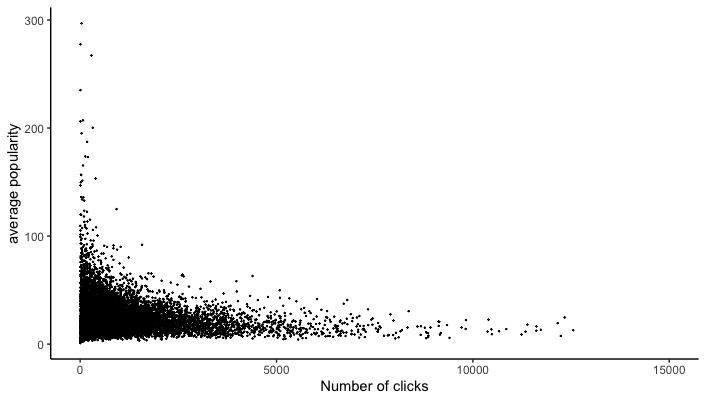
\includegraphics[width=\textwidth]{brand search and item search/graph/Click_popularity.png}
    \caption{Number of clicks versus average popularity}
    \label{fig:emprical_cutoff}
\end{figure}

We now generalize the insight to the markets with multiple designs and restrict our discussion to monotone interval partition thereafter. Denote the set of designs announced by firms at the first stage by $\hat{\S}$ and relabel its elements such that $s_1 < s_2 < \dots < s_n$, where $n$ is the cardinality of set $\hat{\S}$. The lemma/corollary above implies that fixing a price vector $\mathbf{P}%
^{e}_{\hat{\S}}=\left\{ P_{s_1}^{e},P_{s_2}^{e},...P_{s_n}^{e}\right\} $, one of the optimal
search decision takes a monotone interval partition form, given by $\left\{ [a_0,a_{1}),[a_{1},a_{2}),...,[a_{n-2},a_{n-1}),[a_{n-1},a_n]\right\}$, where $[a_0,a_{1})$ is the
interval of search costs that find design $s_1$ (weakly) optimal, $[a_{1},a_{2})$
is the interval of search costs that find design $s_2$ (weakly) optimal, and so
on.\footnote{ A non-degenerated interval of search costs that allows indifference between multiple designs can lead to non-monotone partition.}Note that if no consumer finds design $i$ optimal, the interval $
[a_{i-1},a_{i})$ is empty. Clearly, a monotone interval partition is
characterized by a sequence of nondecreasing cutoffs: $\textbf{a}\equiv \left\{
a_0, a_{1},a_{2},...,a_{n}: a_0=\underline{c} \text{ and } a_n=\bar{c} \right\}$.\footnote{ \label{footnote:cutoff} Define $a_i= \max(a_{i-1}, \min\{\hat{c}_{i,j}, j>i\})$ for $i=1,\dots, n-1$, where $\hat{c}_{i,j}$ is the cutoff between design $s_{i}$ and $s_j$. When $a_{i}=a_{i-1}$, either no consumer find design $i$ (weakly) optimal or precisely consumers with $c=a_i$ are indifferent between multiple designs, e.g. $i-1$,$i$ and $i+1$. We assume none of them search design $i$ in the latter case, so the set of consumers with a specific search mode is either empty or has a positive measure.}


The number of intervals in the monotone partition may be less than the number of announced designs, as searching for some products can be strictly dominated. If every announced design attracts a positive mass of consumers, then we refer to such a collection of designs as an equilibrium design profile, denoted by $\S^*$, and use $\mathbf{\hat{c}}\equiv \{c_1, c_2, \dots, c_n\}$ to represent cutoffs associated with this equilibrium partition. We omit $\mathbf{\hat{c}}$'s dependence on $\S^*$ and $P^e_{\S^*}$ whenever it is clear. The following proposition shows that in the equilibrium, consumers' search strategies are captured by a $n$-interval partition, with the cutoff type being indifferent between adjacent designs.


\begin{prop}\label{prop:partition}
For any $\S^*$, the partition $\mathbf{\hat{c}}$ is chosen in a way that boundary types are indifferent between two neighboring designs.
\begin{equation}\label{eq:partition_characterization}
    \hat{c}_i = \hat{c}(s_{i},s_{i+1}),\qquad \forall i \in \{1,2, \dots, n-1\},\:\text{ and } s_i \in \S^*.
\end{equation}
 That is, 
\begin{equation}\label{eq:boundary_consumer_indifferent}
    v_{s^i}^*(\hat{c}(s_i, s_{i+1}))-v_{s^{i+1}}^*(\hat{c}(s_i, s_{i+1}))= P_{s_i}^e - P_{s_{i+1}}^e.
\end{equation}
\end{prop}

\begin{proof}
We show that consumers in the $i$th interval chooses search mode $i$ if and only if $\hat{c}_i = \hat{c}(s_{i},s_{i+1})$.
For the only if part, we prove by contrapositive. Suppose $\hat{c}(s_{i},s_{i+1})<\hat{c}_i$, consumers with $c$ slightly below $\hat{c}_i$ prefer design $s_{i+1}$ over $s_{i}$, contradicting to the fact that consumers in the $i$ th interval favor design $s_{i}$ over the others. Similarly, if $\hat{c}(s_{i},s_{i+1})>\hat{c}_i$, consumers with search costs slightly above $\hat{c}_i$ lies in the $i+1$ interval but prefer design $s_{i}$ over $s_{i+1}$, contradiction.

For the if part, we first observe consumers in the $k$th interval lies on the right-hand side of $\hat{c}(s_{i}, s_{i+1})$ for $i\in\{1,2,\dots, k-1\}$. Applying the transitivity of consumers' preference, consumers in the $k$th interval prefer design $s_{k}$ to all designs more niche than it. Similarly, since consumers in the $k$th interval lies on the left hand side of $\hat{c}(s_{i}, s_{i+1})$ for $i\in\{k,\dots, n\}$, they prefer design $s^k$ to all broader designs.
\end{proof}
For each $\S^*$ and $P^e_{\S^*}$, there could be multiple $\mathbf{\hat{c}}$ satisfying equation \eqref{eq:partition_characterization} and \eqref{eq:boundary_consumer_indifferent}. As one will see in the later discussion, we will exploit this multiplicity to establish the existence of equilibria.
% \footnote{Another layer of multiplicity concerns the adoption of mixed strategy. Allowing a zero-measure of consumers to mix does not impact demand characterization. } 
The partition structure not only yields an intuitive property on consumers' search behavior but significantly reduces the difficulty in deriving the demand and prices for different designs, which is the objective of the next section.



  

% Combined these indifference conditions with corollary \ref{cor:mixing_and_matching_benefit}, we can derive $P_{s_1}^* \geq P_{s_2}^* \geq \dots \geq P_{s_n}^*$.





\subsection{Firm's strategy }\label{subsection:firm}
In this subsection, we focus on a specific set of equilibrium designs $\S^*$ and abbreviate design $s_k$ as design $k$. 
Define $\mathbf{q}\equiv (q_{1}, q_{2}, \dots, q_{n})$, where $q_{k}$ is the measure of type $k$ firms in the market. We can decompose firms' decision-making into two stages. In the first stage, they commit to a specific design. In the second stage, firms select the optimal prices according to consumers' search behavior solicited by designs chosen in the first stage. Assuming firm $j$ chooses design $k$ in the first stage, we now focus on the second-stage problem. By symmetry, $g(c)dc/q_{k}$ unit of type $k$ shoppers with search costs $c$ come to firm $j$ on their first visit and come to firm $j$ on their second visit whenever they could not find satisfactory products at the first firm, which happens with probability $F_{k}(v_{k}^*(c))$. Since the type-$k$ shoppers purchasing at firm $j$ can visit no, one, two, .... up to an infinite number of firms before, the measure of type-$k$ shoppers with search costs $c$ visiting firm $j$ is $\frac{g(c)dc}{q_{k}\left(1-F_{k}(v_{k}^*(c))\right)}$. Conditional on the visit, the type $k$ shopper stops and purchases at the firm $j$ whenever her actual surplus is higher than the expected surplus ($v_{{k}, j}-P_{{k},j}\geq v_{k}^*(c) - P_{k}^e$). The demand from type-$k$ shoppers with search costs $c$ is thus
%
\begin{equation}\label{eq:demand_s_k}
 D_{k}( P_{{k},j}| \mathbf{P^e}, \mathbf{F^*}, \mathbf{q}, c )dc \equiv \frac{g(c)\left(1-F_{{k}}(v_{k}^*(c)-P_{k}^e+P_{k,j})\right)}{q_k\left(1-F_{k}(v_{k}^*(c))\right)}dc.
\end{equation}
 \footnote{The demand from type $k$ shoppers with $c>\tilde{c_{k}}$ is $\frac{g(c)\left(1-F_{k}(v_k^*(c)-P_k^e+P_{k,j})\right)}{q_k}$. This is because all type $k$ shoppers stop and purchase on their first visit in the equilibrium($v_{k,j} \geq v_k^*(c)$ for all $c>\tilde{c_k}$). Therefore, when firm $j$ encounters type $k$ shoppers with $c>\tilde{c_k}$, it knows with certainty that it must be their first visit.}     Notice that if firm $j$ charges a price $P_{k,j}\geq \bar{v}_{k}-v_k^*(c)+P_k^e$, no consumer with search cost lower than $c'(P_{k,j})$ will stop at firm $j$, where $c'(P_{k,j})$ solves $\bar{v}_{k}-v_k^*(c')+P_k^e-P_{k,j}=0$. Specifically, any price $P_{k,j}> \bar{P_k}(P_k^e)\equiv \bar{v}_{k}-v_k^*(\bar{c})+P_k^e$ prohibits all types of consumers from visiting and is strictly dominated. It is, therefore, without loss to confine the choice set to be $X \coloneqq \{ P_{1,j}, P_{2,j}, \dots, P_{n,j}| P_{k,j}\in [0, \min \left(\bar{v}_k, P_k(P_k^e)\right)] \}$. Since corner solutions yield zero profits, given the belief in equilibrium prices, the optimal pricing strategy for firm $j$ must lie in the interior of this choice set.


From proposition \ref{prop:partition}, the impact of heterogeneous search costs on consumers' search modes can be summarized by equation \eqref{eq:partition_characterization}.  Since the target customers of type-$k$ firms are those with search costs ranging from $\hat{c}_{k-1}$ to $\hat{c}_k$, the profit function of type-$k$ firm is 

\begin{equation}\label{eq:profit_type_k}
 \pi_k(P_{k,j}|\mathbf{P^e}, \mathbf{F^*}, \mathbf{q}) \equiv  P_{k,j}  \int^{\hat{c}_{k}}_{\hat{c}_{k-1}} D_k(P_{k,j}|\mathbf{P^e}, \mathbf{F^*}, \mathbf{q},c )\,dc. 
\end{equation}
If the profit maximization admits an interior solution, $P_k^* =P_k^e$ together with FOC implies
\begin{equation}\label{eq:P_k}
\int_{\hat{c}_{k-1}}^{\hat{c}_k}\bigg[1-P_k^*\frac{f_k(v_k^*(c))}{1-F_k(v_k^*(c))}\bigg]\,dG(c)=0.
\end{equation}
 For all $k\in \S^*$, denote the hazard rate corresponding to distribution $F_k$ by $H_k(v)\equiv \frac{f_k(v)}{1-F_k(v)}$, and the conditional distribution of search costs on the $k$th interval by $\tilde{G}(c;k)\equiv \frac{G(c)-G(\hat{c}_{k-1})}{G(\hat{c}_k)-G(\hat{c}_{k-1})}$ for all $c\in[\hat{c}_{k-1}, \hat{c}_k]$, with $\tilde{g}(c;k) =\tilde{G}'(c;k)$. A necessary condition for $\S^*$ to be sustained as an equilibrium design profile is
\begin{equation} \label{eq:price_candidate}
P_k^*(\S^*) =\frac{1}{\int^{\hat{c}_{k}}_{\hat{c}_{k-1}} H_k(v_k^*(c))\,d\tilde{G}(c; k)}.    
\end{equation} 
The equality indicates that the equilibrium price negatively correlates with the conditional expectation of the hazard rate. To explain the intuition, let's restrict our attention to type-$k$ shoppers with search cost $c$. Because all such shoppers stopping at the firm $j$ obtain expected utility $v_k^*(c)-P_k^*$, a marginal price increase prevents those with valuations equal to the reservation utility from purchasing. Therefore, the marginal consumers accounts for $\frac{f_k(v_k^*(c))}{1-F_k(v_k^*(c))}$ portion of the population eventually buy from firm $j$. Since the target of type-$k$ firms consists of consumers with search costs ranging from $\hat{c}_{k-1}$ to $\hat{c}_k$, $P_k^*=\frac{1}{\H_k(\hat{c}_{k-1}, \hat{c}_k|\S^*)}$ is simply the inverse of the conditional expectation of the hazard rate over the range, where  $\mathcal{H}_k(\hat{c}_{k-1}, \hat{c}_k|\S^* )\equiv \int^{\hat{c}_k}_{\hat{c}_{k-1}} H_k(v_k^*(c))\,d\tilde{G}(c;k)$.  Differentiating the conditional hazard rate with respect to the upper and lower bound, we get 
\[
\frac{\partial \mathcal{H}_k }{\partial \hat{c}_{k}}=\tilde{g}(\hat{c}_{k};k)\left[ H_k(v_k^*(\hat{c}_k)) - \mathcal{H}_k\right]< 0,
\]
and 
\[
\frac{\partial \mathcal{H}_k }{\partial \hat{c}_{k-1}}=\tilde{g}(\hat{c}_{k-1};k)\left[ \H_k- H_k(v_k^*(\hat{c}_{k-1}))\right]< 0.
\]
An upward shift of the lower or the upper bound induces consumers to search less intensively due to higher average search costs; less choosy consumers correspond to a strictly less elastic demand and a higher price.

When will FOC be sufficient for the optimality of price? In the following, we provide two conditions that guarantee the quasi-concavity of the profit function and assume they are satisfied thereafter. One can easily verify that the second-order derivative of the profit function is non-positive if condition (i) holds. Condition (ii) follows directly from Theorem 1 in Moraga-Gonz{\' a}lez et al.(2017). The basic idea is to observe that the demand from a particular consumer is log-concave in the price and the reservation utility under condition (ii). After that, they show that log-concavity is preserved under aggregation by the Prékopa Theorem(1973). Since the profit function is a product of the price and the aggregate demand, the profit function is log-concave and, therefore, quasi-concave.
\begin{ass}\label{ass:profit_sufficiency}
For all $k$ either (i) $f_k'(v_k)\geq 0$ or (ii) $g(v_k^{*-1}(t))$ is log-concave.
\end{ass}



\subsection{equilibrium}
We first point out any equilibrium profile can be fully characterized by $\S^*$, $\mathbf{\hat{c}}$, $\mathbf{q^*}$, and $\mathbf{P^e}$. For each equilibrium design profile $\S^*$, consumers search according to the partition structure given in \eqref{eq:partition_characterization}, and firms set on-path prices according to equation \eqref{eq:price_candidate}, both of which are solely determined by $\mathbf{\hat{c}}$. The product design profile $\mathbf{F^*}$, by ex-ante symmetry of firms, can be equivalently translated into the composition of firms $\mathbf{q^*}$, which is endogenously determined by the profit indifference condition \eqref{eq:profit_indifference}. For each $k,k'\in \S^*$,
\begin{equation}\label{eq:profit_indifference}
\pi_k(P_k^* |\mathbf{P^e}, \mathbf{F^*}, \mathbf{q^*}) = \pi_{k'}(P_{k'}^*| \mathbf{P^e}, \mathbf{F^*}, \mathbf{q^*})=\pi^*(\S^*).
\end{equation}
% Since $\mathbf{q}$ can be scaled proportionally while maintaining the profit-indifference conditions, the existence of $\mathbf{q^*}$ is guaranteed.

Finally, beliefs in the prices of on-path designs should be consistent with the actual prices, and beliefs in the prices of off-path designs should prevent any consumer from exploring it in case appearing at the first stage. As consumers have all the freedom to assign beliefs out of the equilibrium path, setting expected prices of unseen designs to be exceedingly high ensures no consumer is willing to look into them; such an equilibrium exists as long as $\mathbf{\hat{c}}$ and $\mathbf{P^*}$ satisfying equations \eqref{eq:boundary_consumer_indifferent} and \eqref{eq:price_candidate}.\footnote{In particular, any market with a single design $k$ can be sustained as an equilibrium by setting the expected price of an off-path design $j$ to satisfy $P_j^e> v_j^*(\underline{c})-v_k^*(\underline{c})-P_k^*(\{s_k\})$ for all $j<i$ and $P_j^e> v_j^*(\bar{c})-v_k^*(\bar{c})-P_k^*(\{s_k\})$ for all $j<i$. The question is whether this belief is rational.} An important inquiry concerns the rationality of consumer beliefs in off-path designs, specifically whether the firm will indeed adhere to the anticipated price if it adopts an unseen design. Given consumer belief, every price yields zero payoffs, so the firm should be indifferent between them. But is some prices more sensible than others? Firms should certainly exclude some prices from their consideration, such as any price above $\frac{1}{H_k(v_k^*(\bar{c}))}$ or below $\frac{1}{H_k(v_k^*(\underline{c}))}$ because any price within this range cannot be supported by any customer base $\mathcal{A} \subseteq [\underline{c}, \bar{c}]$. Moreover, if a design can attract any consumer, the set of customers must be convex. Given these observations, we can define rational belief formally as follows.
\begin{defn}
A belief system $\mathbf{P^e}$ is rational if for all $k$, there exists a convex set $\mathcal{A}_k\subseteq [\underline{c}, \bar{c}]$ such that $P^e_k$ solves 
\[\max_{[0, \bar{v_k}]} \: p_k\int_{\mathcal{A}_k} \frac{1-F_k(v_k^*(c)-P_k^e+p_k)}{1-F_k(v_k^*(c))}\,dG(c).\]
\end{defn}
Next, we show that an equilibrium exists under a rational belief system and briefly describe the construction, with detail relegated to the appendices. 

\begin{prop}
There exists an equilibrium $(\S^*, \mathbf{\hat{c}}, \mathbf{q^*}, \mathbf{P^e})$ supported by a rational belief.
\end{prop}
The idea is to construct a self-map from the product space of a weakly increasing sequence of cutoffs $\mathbf{a}$ and expected prices $\mathbf{P^e}$ to itself. For any belief in prices, the optimal search decision is captured by a correspondence of weakly increasing cutoffs summarizing the associated monotone interval partition in a fashion similar to footnote \ref{footnote:cutoff}. Firms choose optimal prices according to a sequence of cutoffs and expected prices, assuming consumers between the $k-1$th and the $k$th cutoff search for design $k$. If this interval degenerates, no consumer prefers to search design $k$, and the firm forms its profit maximization problem assuming only consumers with search costs equal to the cutoff pay a visit. Then we show these two correspondences are upper-hemicontinuous, compact-and convex-valued and apply the Kakutani fixed-point theorem to prove the existence. Our next objective is to examine the condition in which multiple designs coexist in the market, known as a separating equilibrium, as well as the situation where a single design dominates, referred to as a pooling equilibrium. To facilitate analysis, we limit our focus to equilibria with a maximum of two designs and outline some key properties.

\subsection{Separating equilibrium ($\lvert \S^* \rvert=2$)}
\begin{lemma}\label{lemm:c_hat_bound}
There exists a separating equilibrium only if $\hat{c}_1< \tilde{c_2}$.
\end{lemma}
\begin{proof}
Suppose towards a contradiction; there exists a separating equilibrium in which all broad shoppers have search costs  $ c\geq\hat{c}_1\geq\tilde{c_2}$. In the equilibrium, almost all broad shoppers except the one with $c=\tilde{c}_2$ will stop and purchase at their first visit, which makes the demand infinitely inelastic locally. Increasing the price of the broad products by $\varepsilon$ is equivalent to shifting consumers' match value downward by $\varepsilon$. The demand from consumers with search costs higher than $c^*(\varepsilon)$ remains intact since these consumers will purchase immediately like before, where $c^*(\varepsilon)$ solves $v_2^*(c^*)+\varepsilon = \underline{v}_2$. On the other hand, the probability of purchasing for consumers with $\tilde{c}_2\leq c<c^*(\varepsilon)$ will decline by $F_2(v_2^*(c)+\varepsilon)$ since now broad shoppers continue to search if $v_2-\varepsilon < v_2^*(c)$. Define $\varepsilon_1 \equiv c^*(\varepsilon)-\tilde{c}_2$. The marginal impact of raising $P_2^*$ by $\varepsilon$ is, therefore, at least $[1-G(c^*(\varepsilon))]\varepsilon-P_2^*\int_{\tilde{c}_2}^{\tilde{c}_2+\varepsilon_1}F_2(v_2^*(c)+\varepsilon)\,dG(c)$. The second term is negligible compared to the first term because $F_2(v_2^*(c)+\varepsilon)<F_2(\underline{v_2}+\varepsilon)<\varepsilon_2$ for $\varepsilon_2>0$, implying raising price by $\varepsilon$ is profitable.
\end{proof}
The equilibrium prices are determined by three factors: the dispersion effect, the location effect, and the compositional effect.
For any fixed $v$, and $s'<s$, $H_{s'}(v)\leq H_{s}(v)$. This result comes from theorem 2.1 of Khaledi (2002), stating that under increasing failure rate(which is ensured by assumption \ref{ass:logconcave_f}), dispersed order implies hazard rate order. Since the hazard rate corresponds to the portion of marginal consumers susceptible to an increase in price, a higher hazard rate is associated with more elastic marginal demand and a lower price. The first force, named the dispersion effect, makes standardized products cheaper. Second, the position of the marginal consumers in the distribution varies for different search modes. Suppose all consumers have search costs $c$; niche shoppers have higher reservation utilities due to greater mixing and matching benefits. Given the same product design, the demand from niche shoppers is closer to the upper tail of the distribution and hence is more elastic. We term this the location effect.
The compositional effect captures the difference in search costs between niche and broad shoppers, that is, the domain of search costs which the hazard rate function integrates over. As broad shoppers are composed of consumers with high search costs, firms have a higher local monopoly power over standardized products. In other words, the search-discouraging impact is stronger for broad shoppers assuming the same valuation distribution. Mathematically, $H_k(v_k^*(c))$ is a non-increasing function of $c$, suggesting the demand from high-cost shoppers is less elastic. In summary, the dispersion effect works opposite to the compositional and the location effect in the direction of raising (reducing) the elasticity of the broad (niche) products.

The following lemma states that the dispersion effect should dominate the combination of the location effect and composition effect, leading to higher prices for niche products. Essentially, a firm can charge a higher price for the niche product because it caters to consumers' tastes better than the generic product, captured by $v_1^*(c)\geq v_2^*(c)$ for all $c$.

\begin{lemma}
A niche product is no cheaper than a standardized product, and the number of consumers per firm is higher for standardized products.
\end{lemma}
\begin{proof}
From the consumer's indifference condition and corollary \ref{cor:mixing_and_matching_benefit}, we know the price of a niche product must be no lower than a standardized product. The second part of the statement follows directly from the profit-indifference condition.
\end{proof}

\begin{cor}
For any $\S^*$, $H_1(v_1^*(\hat{c}_1))<H_2(v_2^*(\hat{c}_1))$.
\end{cor}
\begin{proof}
From the previous lemma, we understand the dispersion effect works against and dominates the other two effects. Observing the dispersion effect outweighs the location effect in the absence of the composition effect completes the proof. Mathematically, \[\frac{1}{H_1(v_1^*(\hat{c}_1))}>P_1^*=\frac{1}{\H_1(\underline{c},\hat{c}_1|\S^*)}>P_2^* = \frac{1}{\H_2(\hat{c}_1, \bar{c}|\S^*)}>\frac{1}{H_2(v_2^*(\hat{c}_1))}.\]
\end{proof}
The corollary positions that the dispersion effect dominates the location effect for cutoff-type consumers. In general, it's hard to check whether the condition is satisfied due to difficulty in calculating the reservation utility. However, it's easy to verify the condition holds for all $c$ if the valuation density is uniform.\footnote{Consider uniform valuation distribution $F(v;\gamma)$ with mean $\frac{1}{2}$ over the support $[\frac{1-\gamma}{2}, \frac{1+\gamma}{2}]$, where $\gamma$ measures the level of dispersion. Let $X_{\gamma}$ be the random variable associated with distribution $F(v;\gamma)$. One can easily verify $X_{\gamma}\leq_{\text{disp}}X_{\gamma'}$if $\gamma'>\gamma$. Define the hazard rate of $X_{\gamma}$ by $H_\gamma$ and the reservation utility by $v_{\gamma}^*$. $H_\gamma(v_{\gamma}^*(c))=\frac{1}{\sqrt{2\gamma c }}$, which is a decreasing function of $\gamma$. }
Now we are ready to provide a sufficient condition for the existence of $\hat{c}_1$. Define $h(\hat{c}_1|S^*)\equiv v_1^*(\hat{c}_1)-v_2^*(\hat{c}_1)-P_1^*(\hat{c}_1)+P_2^*(\hat{c}_1)$ as the change in consumer surplus when the cutoff type switch from searching the broad design to the niche design. Since the difference between the reservation utility is non-increasing in search costs, $h(\hat{c}_1|\S^*)$ decreases with $\hat{c}_1$ if $P_1^*-P_2^*$ is increasing. 
The slope of the price difference is given by
\[
\frac{d}{d \hat{c}_1}(P_1^*-P_2^*) = -\frac{g(\hat{c}_1)[H_1(v_1^*(\hat{c}_1))-\H_1]}{\H_1^2G(\hat{c}_1)}+\frac{g(\hat{c}_1)[\H_2-H_2(v_2^*(\hat{c}_1))]}{\H_2^2[1-G(\hat{c}_1)]}
\]
Therefore, $h(\hat{c}_1|\S^*)$ is decreasing if 
\[
 \lvert\frac{d P_1^*}{d \hat{c}_1}\big/\frac{d P_2^*}{d \hat{c}_1}\rvert=\frac{\H_2^2[H_1(v_1^*(\hat{c}_1))-\H_1]}{\H_1^2 [\H_2-H_2(v_2^*(\hat{c}_1))]}\times \frac{1-G(\hat{c}_1)}{G(\hat{c}_1)}>1.
\]
Since the first term is positive, the condition holds if there is not much density accumulating in the low-cost region or $g(c)$ is an increasing and sufficiently convex function. In what follows, we show a unique separating equilibrium exists if $G(\tilde{c}_2)$ is small enough. Intuitively speaking, an upward shift of the cutoff would induce median-cost shoppers to switch from searching for niche products to generic products. When the density of low-cost consumers is insignificant compared to that of high-cost consumers, this change in extensive margin introduces a greater proportion of median-cost consumers to enter the market for niches than to exit the market for generics. That is to say, the search-discouraging effect intensifies more for the niche product, causing $P_1^*-P_2^*$ to decrease arbitrarily fast with the cutoff. The condition $\underline{c}=0$ ensures that the price of the niche product is sufficiently low, so consumers with the lowest search costs prefer to be niche shoppers. The proof holds through as long as the search costs of the lowest type satisfy
$\lim_{\hat{c}_1\to\underline{c}}h(\hat{c}_1|\S^*)>0$.


\begin{prop}\label{prop: separating_eq_existence}
Suppose $\underline{c}=0$, there exists a $k^*$, such that there is a unique separating equilibrium if $G(\tilde{c}_2)<k^*$.
\end{prop}
\begin{proof}
We first focus on the case where $\tilde{c_2}<\bar{c}$.
Since $G(c)$ has no atom, $\H_i^2$, and  $H_i(v_i^*(c))-\H_i$ are both bounded above and below. There exists $\varepsilon>0$, such that \[\frac{\H_2^2[H_1(v_1^*(\hat{c}_1))-\H_1]}{\H_1^2 [\H_2-H_2(v_2^*(\hat{c}_1))]}>\varepsilon,\: and -\frac{g(\hat{c}_1)[H_1(v_1^*(\hat{c}_1))-\H_1]}{\H_1^2}>\varepsilon.\] 
Setting $G(\tilde{c_2})<k^*=\min(\frac{\varepsilon}{2+\varepsilon}, \frac{\varepsilon\tilde{c}_2}{2[\bar{v}_1-\bar{v}_2+P_2^*(0)]})$ ensures $\lvert\frac{d P_1^*}{d \hat{c}_1}\big/\frac{d P_2^*}{d \hat{c}_1}\rvert >2$ and therefore implies for all $\hat{c}_1< \tilde{c}_2$,
\[
\frac{d}{d \hat{c}_1}(P_1^*-P_2^*)>\frac{1}{2}\frac{d}{d \hat{c}_1}P_1^* = -\frac{g(\hat{c}_1)[H_1(v_1^*(\hat{c}_1))-\H_1]}{2\H_1^2G(\hat{c}_1)}>\frac{\varepsilon}{2G(\hat{c}_1)}> \frac{\bar{v}_1-\bar{v}_2+P_2^*(0)}{\tilde{c}_2}.
\]
If $G(\hat{c}_2)<k^*$, we have
\[
\lim_{\hat{c}_1 \to \tilde{c}_2}h(\hat{c}_1|\S^*) = h(0|\S^*) + \int_0^{\tilde{c}_2}\frac{d h(\hat{c}_1|\S^*)}{d\hat{c}_1}\,d\hat{c}_1\leq \bar{v}_1-\bar{v}_2+P_2^*(0)- \int_0^{\tilde{c}_2}\frac{d P_1^*-P_2^*}{d\hat{c}_1}\,d\hat{c}_1<0,
\]
and
\[\lim_{\hat{c}_1 \to 0} h(\hat{c}_1|\S^*)= \bar{v}_1 -\bar{v}_2 + P_2^*(0)>0.\]
Here $\bar{v}_1-\bar{v}_2>0$ follows from the property that the support of $v_2$ is a strict subset of the support of $v_1$.
By the intermediate value theorem, there exists a $\hat{c}_1^*$ solving $h(\hat{c}_1|\S^*)=0$. The uniqueness follows from the fact that $h(\hat{c}_1|\S^*)$ is decreasing on $[0,\tilde{c}_2]$.
Proof for the case of $\bar{c}<\tilde{c}_2$ is similar by observing the slope of $h(\hat{c}_1|\S^*)$ can be made arbitrarily negative.
\end{proof}
One may wonder whether the assumption that the proportion of low-cost consumers is small meets real-life situations. As indicated by graph \ref{fig:emprical_cutoff}, the majority of users accumulate at the left part; and as the number of clicks increase(corresponding to lower search costs), the density becomes more and more sparse. The data set shows that most of the users click no more than 5000 times, and only 256 out of 10000 users sampled more than that, suggesting condition stated in the hypothesis of proposition \ref{prop: separating_eq_existence} is likely to be met in this particular example.




 The next result shows that pooling equilibrium with the most niche design generates the highest profit. 
\begin{lemma}\label{lemma:eq_refinement_payoff}
Let $\S^*$ be any design profile of a separating equilibrium,  $\pi^*(\{s_1\})>\pi^*(\S^*)$, where $s_1$ is the most niche design in $\S^*$.
\end{lemma}
\begin{proof}
\[\pi^*(\{s_1\})=P_1(\{s_1\})>P_1(\S^*)\geq\sum_{i=1}^n P_i^*(\S^*)[G(\hat{c}_i)-G(\hat{c}_{i-1})]=\pi^*(\S^*).\]
The first inequality follows from the fact that only consumers with the lowest search costs choose the most niche design in a separating equilibrium, in contrast with the pooling equilibrium, where firms target the whole spectrum of buyers.
\end{proof}


% \noindent \textbf{Equilibrium Refinement}

% Since there could be multiple equilibria, one natural question is which one is more likely to happen. The next lemma shows that the equilibrium with fewer designs is payoff-dominant.









 








\section{Comparative statics ($\lvert\S \rvert = 2$)}\label{section:comparative statics}
In this section, we parameterize the distribution of search costs by a positive number $\beta$. Specifically, denoting the parametrized CDF by $G(c; \beta)$ and denote the corresponding pdf by $g(c, \beta)$ defined over the support $[\underline{c}, \bar{c}]$. Here we assume the support does not depend on $\beta$ so as to isolate the effect of an endogenous shift of the cutoff. Furthermore, we denote the conditional distribution of $c$ truncated above at $\hat{c}_1$ by $\bar{G}(c;\beta, \hat{c}_1 )$, the counterpart truncated below at $\hat{c}_1$ by $\underline{G}(c;\beta,\hat{c}_1)$, with density $\bar{g}(c;\beta, \hat{c}_1 )$ and $\underline{g}(c;\beta, \hat{c}_1 )$ respectively.  $G(c;\beta)$ is continuously differentiable with  $\beta$. With this definition, the conditional hazard rates of niche shoppers and broad shoppers are given by  $\H_1(\underline{c}, \hat{c}_1;\beta) = \int^{\hat{c}_1}_{\underline{c}}H_1(v_1^*(c))\,d\bar{G}(c,\hat{c}_1;\beta)$ and $\H_2(\hat{c}_1, \bar{c};\beta) = \int_{\hat{c}_1}^{\bar{c}}H_2(v_2^*(c))\,d\underline{G}(c,\hat{c}_1;\beta)$ respectively. The objective is to study how changes in the distribution of search costs affect the cutoff and equilibrium prices.
\begin{defn}
Search costs decrease with $\beta$ in the FOSD sense if $G(c; \beta)\leq G(c;\beta')$ for all $c$ and $\beta'\leq \beta$. i.e. $G_{\beta}(c;\beta)\leq 0$ for all $c$ with strict inequality for some $c$.
\end{defn}
\noindent An equivalent definition of FOSD is that for every non-decreasing function $u:\R\to \R$, $\int u(x)\,dG(c;\beta)\geq \int u(x)\, dG(c;\beta')$. This alternative definition helps proving the next result.
\begin{lemma}
In the pooling equilibrium, a FOSD decrease in search costs reduces the equilibrium price. i.e. $P_s(\beta')\leq P_s(\beta)$ for all $\beta'<\beta$.
\end{lemma}
\begin{proof}
Since $H_s(v_s^*(c))$ is non-increasing in $c$, 
 we have for all $\beta>\beta'$,
\[\int^{\Bar{c}}_{\underline{c}}H_s(v_s^*(c))\,dG(c;\beta)\leq \int^{\Bar{c}}_{\underline{c}}H_s(v_s^*(c))\,dG(c;\beta').\]
Taking the reciprocal of the inequality completes the proof.
\end{proof}
In a separating equilibrium, the cutoff $\hat{c}_1^*(\beta)$ changes with the distribution of search costs, and solves 
\[
L(\hat{c}_1, \beta) \equiv v_1^*(\hat{c}_1)-v_2^*(\hat{c}_1)-\frac{1}{\H_1(\underline{c},\hat{c}_1;\beta)}+\frac{1}{\H_2(\hat{c}_1,\bar{c};\beta)}=0.
\]
Provided $\frac{\partial f}{\partial \hat{c}_1}\neq 0$ at the equilibrium cutoff $\hat{c}_1^*(\beta)$, the implicit function theorem suggests the effect of a marginal decrease in $\beta$ on the cutoff is 
\[
\frac{d\hat{c}_1^*(\beta)}{d \beta} = -\frac{\frac{\partial L(\hat{c}_1^*(\beta),\beta)}{\partial \beta }}{\frac{\partial L(\hat{c}_1^*(\beta),\beta)}{\partial \hat{c}_1 }}.
\]
By proposition \ref{prop: separating_eq_existence}, the denominator is negative given there are sufficiently many high-cost consumers. 
The sign of $\frac{d \hat{c}_1^*(\beta)}{d \beta}$ therefore depends on the sign of $\frac{\partial L(\hat{c}_1), \beta)}{\partial \beta}$ at the equilibrium cutoff, which is
\begin{equation}\label{eq:comparative_statics_cutoff}
\frac{1}{(\H_1)^2} \frac{\partial}{\partial \beta} \H_1(\underline{c},\hat{c}_1;\beta)
 - \frac{1}{(\H_2)^2} \frac{\partial}{\partial \beta} \H_2(\hat{c}_1,\bar{c};\beta) \bigg\vert_{\hat{c}_1 = \hat{c}_1^*}.
\end{equation}
Once the sign of $\frac{d \hat{c}_1^*(\beta)}{d \beta}$ is obtained, we can use it to derive the comparative statics of equilibrium prices. As the equilibrium price is inversely proportional to the conditional hazard rate, we focus on how search costs affect the latter. A marginal decrease in search costs affects the equilibrium prices in two ways, which can be seen clearly from the derivative of the conditional hazard rate given by
\begin{equation}\label{eq:comparative_P1}
\frac{d}{d \beta} \H_1 = \bar{g}(\hat{c}_1^*;\hat{c}_1^*,\beta) \left[H_1(v_1^*(\hat{c}_1^*(\beta)))-\H_1\right]\frac{d \hat{c}_1^*(\beta)}{d\beta} + \frac{\partial \H_1 }{\partial \beta}.
\end{equation}
The first term is the compositional effect (extensive margin), an endogenous shift of the cutoff induces consumers to join or drop out of the market of niches. In the case that $\frac{d \hat{c}_1^*(\beta)}{d\beta}<0$, a decrease in the search cost would incentivize marginal consumers originally purchasing standardized products to switch to niches. As these newcomers have higher search costs, the compositional effect tends to reduce the average elasticity and raise the price of niche products. The second term captures the search-discouraging effect (intensive margin), which is equivalent to change in the conditional distribution of search costs in the absence of a cutoff change, indicating the average search intensity had the cutoff remain unchanged. Similarly, the price decomposition for standardized products is 
\begin{equation}\label{eq:comparative_P2}
\frac{d}{d \beta}\H_2 = \underline{g}(\hat{c}_1^*;\hat{c}_1^*,\beta)\left[\H_2-H_2(v_2^*(\hat{c}_1^*(\beta))) \right] \frac{d\hat{c}_1}{d\beta}+ \frac{\partial \H_2}{\partial \beta}.
\end{equation}
In general, it is hard to determine the sign of the search-discouraging effect, equivalently, whether a FOSD decrease of the distribution of search costs would result in a FOSD decrease of the distribution truncated from above (below). Proposition 3 and 4 of Moraga-Gonz{\' a}lez et al.(2017) show that the statement is true if the density has the increasing likelihood ratio property (ILRP) and the reserve result--- a FOSD decrease leads to a FOSD increase of the distribution truncated above--- is valid under decreasing likelihood ratio property(DLRP). Nonetheless, how cutoff changes is determined by the relative magnitude of the search-discouraging effect between two markets. Therefore, knowing the direction of the change of the stochastic ordering is insufficient to pin down the comparative statics of either the cutoff or prices. As a simplification, below we focus on two special cases where the search discouraging effect is absent for one market ($\frac{\partial \H_k}{\partial \beta}=0$ for either $k=1$ or $k=2$). These special settings allow us to derive unambiguous comparative statics.





% In the following, we first build the connection between ILRP (DLRP) and FOSD of the truncated distribution, then discuss the comparative statics of the separating equilibrium consisting of only two designs. i.e., $\lvert \S ^* \rvert=2$.
% \begin{lemma}\label{lemm:IRLP_DRLP}
% For all $\beta' > \beta$,\leavevmode
% \begin{enumerate}
%     \item [(i)] If $g(c;\beta)$ satisfies the ILRP, then $\bar{G}(c; \beta', \hat{c})$ first-order stochastic dominates $\bar{G}(c; \beta, \hat{c})$ for $\hat{c} \leq \min\{ \bar{c}(\beta), \bar{c}(\beta') \}$. Furthermore, if $\bar{c}(\beta)$ is independent of $\beta$, then $\underline{G}(c; \beta', \hat{c})$ first-order stochastic dominates $\underline{G}(c; \beta, \hat{c})$. 
%     \item [(ii)]If $g(c;\beta)$ satisfies the DLRP, then $\bar{G}(c; \beta, \hat{c})$ first-order stochastic dominates $\bar{G}(c; \beta', \hat{c})$ for $\hat{c} \geq \min\{ \underline{c}(\beta), \underline{c}(\beta') \}$.  Furthermore, if $\bar{c}(\beta)$ is independent of $\beta$, then $\underline{G}(c; \beta, \hat{c})$ first-order stochastic dominates $\underline{G}(c; \beta', \hat{c})$.
% \end{enumerate}
% \begin{proof}
% The part related to the search costs distribution truncated above follows directly from Proposition 3 and 4 in Moraga-González et al(2017). Following their method, we prove the counterpart related to the distribution truncated from below. We first prove the case of DLRP. For $\bar{c}\geq d \geq x \geq c\geq \hat{c}\geq \min\{ \underline{c}(\beta), \underline{c}(\beta') \}$
% \begin{align*}
%     &\int ^{x}_{\hat{c}} g(c; \beta) g(d;\beta')\, dc \geq \int ^{x}_{\hat{c}} g(c, \beta') g(d, \beta)\, dc\\
%     \implies& \left[G(x; \beta) - G(\hat{c}; \beta)\right]g(d;\beta') \geq \left[G(x; \beta') - G(\hat{c}; \beta')\right]g(d, \beta)\\
%     \implies& \left[G(x; \beta) - G(\hat{c}; \beta)\right]\int ^{\bar{c}}_{\hat{c}}g(d;\beta')\,dc \geq \left[G(x; \beta') - G(\hat{c}; \beta')\right]\int ^{\bar{c}}_{\hat{c}}g(d, \beta)\,dc\\
%     \implies& \left[G(x; \beta) - G(\hat{c}; \beta)\right]\left[1- G(\hat{c};\beta')\right]\geq \left[G(x; \beta') - G(\hat{c}; \beta')\right]\left[1- G(\hat{c};\beta)\right]\\
% \end{align*}
% Reversing all the inequality proves the case for ILRP.
% \end{proof}

% \end{lemma}
\begin{prop}
Let $\hat{c}_1^*(\beta)$ be the unique separating equilibrium cutoff corresponding to density $g(c; \beta)$. Provided a unique equilibrium exists for a small perturbation around $\beta$, we have the following.
\begin{enumerate}
    \item[(i)] If a FOSD decrease (increase) in search costs does not affect distribution above $\hat{c}_1^*(\beta)$, the change results in a higher (lower) cutoff and higher (lower) prices for standardized products. The price response of niches is ambiguous.
    \item[(ii)] 
    If a FOSD decrease (increase) in search costs does not affect distribution below $\hat{c}_1^*(\beta)$, the change results in a lower (higher) cutoff, lower (higher) prices for both niches and standardized products.
\end{enumerate}
\end{prop}

\begin{proof}
Under condition (i), we have $\frac{\partial \H_1 (\underline{c},\hat{c}_1^*;\beta)}{\partial \beta}\leq 0$ and $\frac{\partial \H_2 (\hat{c}_1^*, \bar{c}; \beta)}{\partial \beta} =0$ by the definition of FOSD of the distribution truncated above. Equation \eqref{eq:comparative_statics_cutoff} reveals the cutoff rises with a marginal decrease in $\beta$($\frac{d\hat{c}_1^*(\beta)}{d\beta}\leq 0$). Since $\H_2(v_2^*(c))$ is non-increasing, $\H_2 -\H_2(v_2^*(\hat{c}_1^*(\beta)))\leq 0$. Equation \eqref{eq:comparative_P2} then implies that in the absence of the search discouraging effect, the compositional effect lowers the conditional hazard rate and drives up the prices of standardized products. The impact on niche products is ambiguous since the compositional effect works against the search-encouraging effect. If the mass of consumers switching their search behavior is substantial, the newly join high-cost niche shoppers could more than counteract the reduction of search costs in the low-cost region, leading to higher prices of  niche products. 
Under condition (ii), we have $\frac{\partial \H_1 (\underline{c},\hat{c}_1^*;\beta)}{\partial \beta}= 0$, $\frac{\partial \H_2 (\hat{c}_1^*, \bar{c}; \beta)}{\partial \beta} \leq0$, and $\frac{d\hat{c}_1^*(\beta)}{d\beta}\geq 0$.When search costs decline in the upper part of the distribution, standardized products become cheaper, which induces more consumers to search for blockbusters, therefore shifting the cutoff downwards. Only the compositional effect is in play for niches; as those medium-cost consumers change to purchasing standardized products, the average search costs of niche shoppers decrease, leading to lower prices. For the standardized product, the result is unambiguous since the two effects work in the same direction. A decline in search costs for those with high search costs intensifies the price competition for standardized products and induces more median-cost consumers to join the generic market. As the demand from these consumers is relatively elastic compared to those originally in the market, the compositional effect reinforces the search discouraging effect, making the competition more fierce.
\end{proof}

The above proposition implies the group of people enjoying an improvement in search technology matters for the price response. Suppose heterogeneity in search costs is due to accessibility to the internet. For instance, the old generation may go to a supermarket physically if they want to do grocery shopping, whereas the young generation can submit their order through an e-commerce platform. If the improvement occurs mainly for consumers with low search costs, such as the introduction of a recommendation engine. In that case, the effect is likely anti-competitive(especially when the extensive margin plays a crucial role). In contrast, a more efficient retail display or better traffic control is pro-competitive. With this observation, we contend that companies may use more obfuscation offline than online. The implication is particularly important as the parallel operation on both markets gains increasing popularity. Two examples are Amazon's acquisition of Whole Foods Markets and Walmart's purchase of Jet.com.



\section{Conclusion}\label{section:conclusion}
In this paper, we study how search costs influence product designs through the demand channel and demonstrate the negative relationship between search costs and designs carried over to an individual level. Our first contribution is to provide a theoretical framework to model how search friction affects consumers' preferences toward different designs. The assumption of dispersive ordering provides a tractable partition structure that allows us to simplify the demand and equilibrium characterization. Empirically, a tendency toward niche products for consumers with low-search costs is verified from the e-commence data provided by Taobao. Our second contribution is to offer another justification for the unconventional price response in addition to the previous literature (Chen and Zhang 2011, Zhou 2014, MorMoraga-Gonz{\' a}lez et al. 2017, Choi et al. 2018). When search costs decrease, medium-type consumers could endogenously switch from seeking generics to niches, raising the average search intensity and prices in both markets. Specifically, we highlight that reduction in search costs can have either pro-competitive or anti-competitive effects depending on the distribution's shape, implying that obfuscation can harm firms in some cases.

Finally, our model can be applied to the study of bundling. Given that a bundle is more dispersed than the item, our first result indicates consumers with low-search costs incline towards purchasing individual items separately. This is in line with Harris et al.(2006), in which they show experimentally that subjects with less motivation to process information have a stronger preference toward bundles.

\section{Example}\label{section: example}
\subsection{Uniform valuation with a ploynomial cost function}
In the following, we assume $F_1(v_1) =v_1$ for $v_1\in [0,1]$, and $F_2(v_2)= 2(v_2-\frac{1}{2}) + \frac{1}{2}$ for $v_2 \in [\frac{1}{4}, \frac{3}{4}]$. Let $G(c) = (\frac{c}{\Bar{c}})^{\alpha}$ for $c\in [0, \Bar{c}]$, where $ \Bar{c}= \tilde{c_2} = \frac{1}{4}$. The reservation utilities of a niche and a standardized product are $v_1^*(c)=1-\sqrt{2c}$ and $v_2^*(c)=\frac{3}{4}-\sqrt{c}$, respectively.
FOC is sufficient to pin down the optimal pricing strategy because $f_i'(v)=0$ for $i=1, 2$.

By proposition \ref{prop: separating_eq_existence},
there exists a unique separating equilibrium if $\alpha$ is sufficiently large. Specifically, there exists a equilibrium if there is a $\hat{c}\in [0,1/4]$ such that $v_1^*(\hat{c})-v_2^*(\hat{c})-P_1^*(\hat{c})+P_2^*(\hat{c})=0$. Plugging the equilibrium price in \eqref{eq:price_candidate} into the expression gives
\[h(\hat{c};\alpha)\equiv
\frac{\sqrt{\hat{c}}(2\alpha-1)((4\hat{c})^\alpha-1)}{2\alpha\left((4\hat{c})^{\alpha}-2\sqrt{\hat{c}}\right)}.
\]
Evaluating the limit at $\hat{c}=1/4$ gives 
\[
\frac{1}{2} -\frac{(2\alpha -1)}{2\sqrt{2}a}+(3/4-\sqrt{\frac{1}{2}}).
\]
Using the same logic in the proof of proposition \ref{prop: separating_eq_existence}, a separating equilibrium exists for $\alpha>\frac{\sqrt{2}}{4\sqrt{2}-5}\approx 2.15$. The uniqueness of the equilibrium cannot be proved formally due to analytical intractability. However, we can numerically show $h_1(\hat{c},\alpha)<0$ for all $0\leq\hat{c}\leq \frac{1}{4}$ and $2.5<\alpha<6$ by the MATLAB, suggesting for each $\alpha$, there is a unique cutoff $\hat{c}$.

Figure \ref{fig:ex1_eq_price} shows that a FOSD increase in the search cost lowers the prices of both niche and broad products for $\alpha \in [2.5, 3.15]$, whereas the change leads to an increase in the niche price and a decrease in broad price for $\alpha \in [3.15, 6]$. To disentangle the reason behind the unconventional price response in the former case, we define $\hat{c}=0.2$ as the benchmark and compare the price changes with and without the compositional effect. If $\alpha = 3.45$, the actual equilibrium cutoff coincides with the benchmark cutoff, and the equilibrium prices equal the hypothetical prices without an endogenous shift of consumers' search behavior. Since $g(c;\alpha)$ satisfies the increasing likelihood ratio property, an increase in $\alpha$ implies a FOSD increase in the conditional distribution truncated above and truncated below by theorem 1.C.6 in Shaked and Shanthikumar (2007). Therefore, in the absence of change in the cutoff, the search-discouraging effect prevails, resulting in higher prices for both designs, as shown by the dotted line.
 
In contrast, when the cutoff is endogenous, an increase in $\alpha$ causes the price of a niche product to rise more than a standardized product, rendering generic designs more attractive. From figure \ref{fig:ex1_compostional_change}, the proportion of niche shoppers decreases with $\alpha$ over the whole domain. When this countervailing force from the compositional change dominates the search discouraging effect, equilibrium prices could fall with search costs as opposed to conventional wisdom.
\begin{figure}[h!]
    \centering
     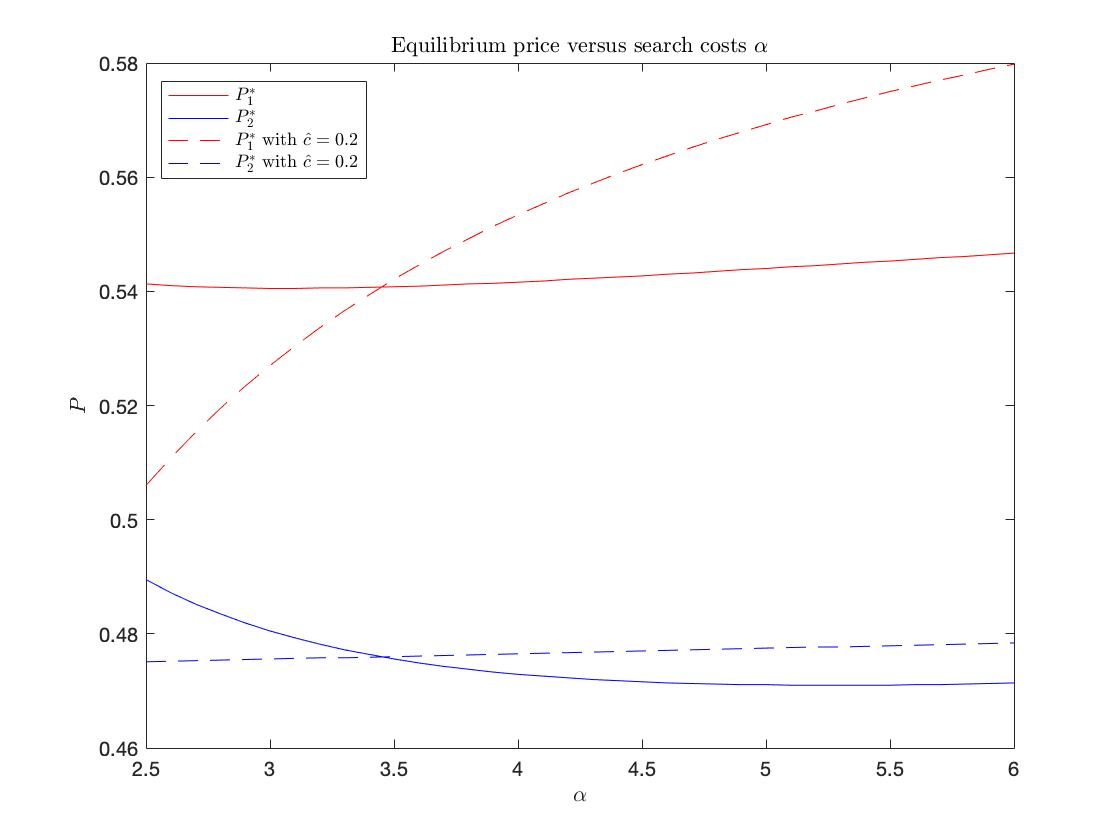
\includegraphics[width = 0.6\textwidth]{brand search and item search/graph/composition_change.jpg}
    \caption{ Equilibrium prices with and without the compositional effect}
    \label{fig:ex1_eq_price}
\end{figure}
\begin{figure}[h!]
    \centering
    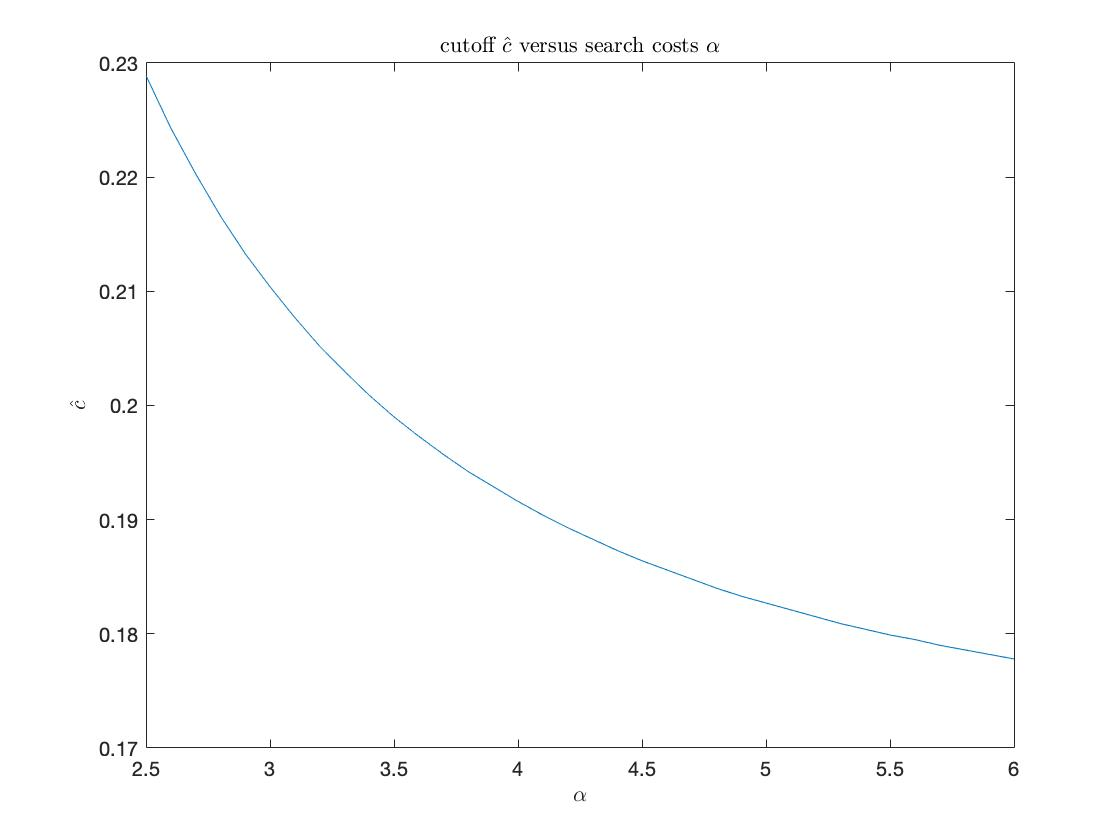
\includegraphics[width = 0.6\textwidth]{brand search and item search/graph/cutoff.jpg}
    \caption{Cutoff versus search costs}
    \label{fig:ex1_compostional_change}
\end{figure}

\begin{figure}[h!]
    \centering
    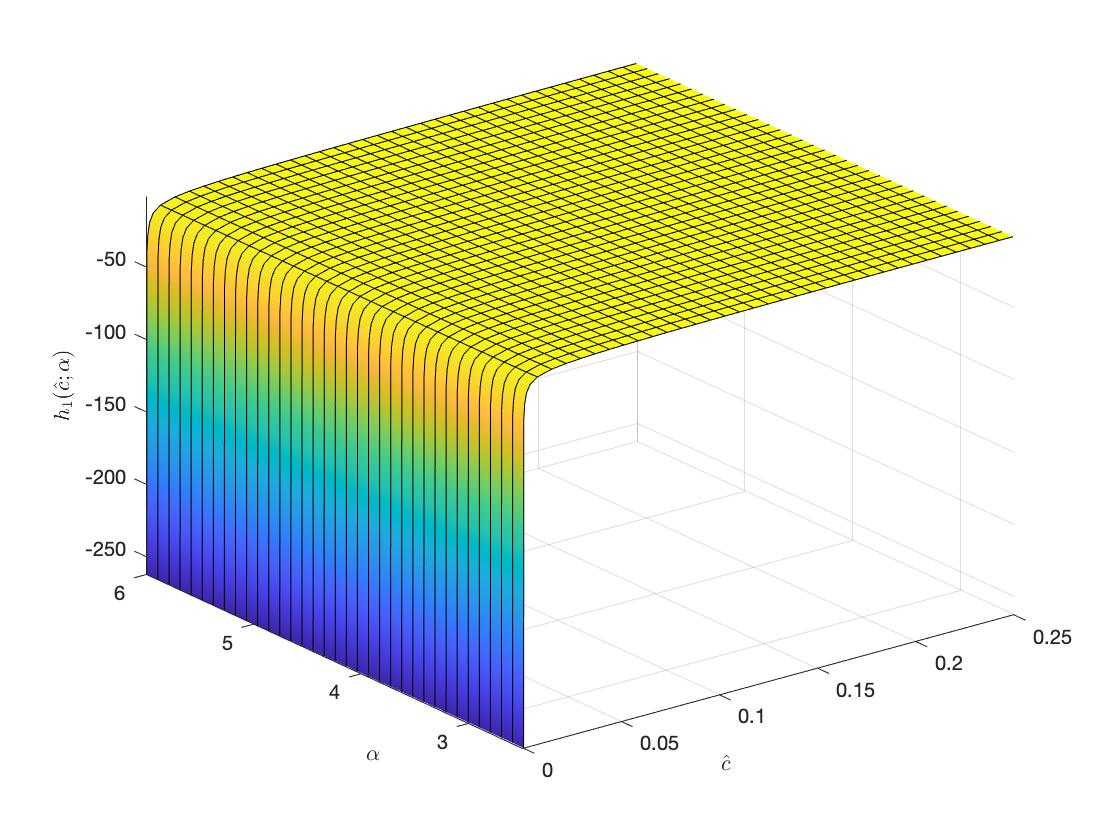
\includegraphics[width = 0.6\textwidth]{brand search and item search/graph/uniqueness.jpg}
    \caption{First order derivative with respect to cutoff}
    \label{fig:ex1_FOD}
\end{figure}






 



\cleardoublepage
%Our appendix starts here
\appendix


\section{Appendix}

\begin{defn}
A correspondence $\Gamma:X\rightrightarrows Y$ is upper-hemicontinuous at $x$ 
if and only if for every sequence $x_{\bullet}=(x_n)_{n=1}^{\infty}\in X$, $y_n\in \Gamma(x_n)$ with $x_{\bullet} \to x$ and $y_{\bullet}=(y_n)_{n=1}^{\infty} \to y\in Y$, we have $y\in \Gamma(x)$.
\end{defn}

Denote the set of all sequences associated with a monotone interval partition by $
K\equiv \left\{ \left\{ a_{1}..,a_{N-1}\right\} \in \left[ \underline{c},\bar{%
c}\right] ^{N-1}:a_{1}\leq a_{2}\leq ...\leq a_{N-1} \right\} $. We first construct the consumer's best response in terms of search decisions.
Let $P=\prod_{k=1}^{N}\left[ 0,\bar{v}_{k}\right] $ be the product price
space. Define a correspondence $\mathbf{C}:P\rightrightarrows \left[ 
\underline{c},\bar{c}\right] ^{\frac{1}{2}N\left( N-1\right) }$ as follows. For each $\mathbf{P}^{e}\in P$, one can construct sequences of cutoffs \[\mathbf{\hat{c}}=\left\{ \hat{c}_{ij}\in \left[ \underline{c},\bar{c}\right]
: i<j\text{ and } i,j=\\ 1,2,...,N\right\} \in \left[ \underline{c},\bar{c}\right]
^{\frac{1}{2}N\left( N-1\right) } \]
satisfying the following condition.
\begin{itemize}
\item If $v_{i}^{\ast }\left( c\right) -P_{i}^{e}=v_{j}^{\ast }\left(
c\right) -P_{j}^{e}$ for some $c\in \left[ \underline{c},\bar{c}\right] $,
set $\hat{c}_{ij}$ to be any one of the solution.

\item If $v_{i}^{\ast }\left( c\right) -P_{i}^{e}>v_{j}^{\ast }\left(
c\right) -P_{j}^{e}$ for all $c\in \left[ \underline{c},\bar{c}\right] $,
set $\hat{c}_{ij}=\bar{c}$.

\item If $v_{i}^{\ast }\left( c\right) -P_{i}^{e}<v_{j}^{\ast }\left(
c\right) -P_{j}^{e}$ for all $c\in \left[ \underline{c},\bar{c}\right] $,
set $\hat{c}_{ij}=\underline{c}$.
\end{itemize}

Denote by $\mathbf{C}\left( \mathbf{P}^{e}\right) $ the set of cutoff
sequences consistent with the conditions above. That is, for each pair $%
i,j=1,2,...,N$ with $i<j$, 

\begin{equation*}
\mathbf{C}_{ij}\left( \mathbf{P}^{e}\right) =\left\{ 
\begin{array}{cc}
\left\{ \bar{c}\right\}  & \text{if }v_{i}^{\ast }\left( c\right)
-P_{i}^{e}>v_{j}^{\ast }\left( c\right) -P_{j}^{e}\text{ for all }c\in \left[
\underline{c},\bar{c}\right] \\ 
\left\{ \underline{c}\right\}  & \text{if }v_{i}^{\ast }\left( c\right)
-P_{i}^{e}<v_{j}^{\ast }\left( c\right) -P_{j}^{e}\text{ for all }c\in \left[
\underline{c},\bar{c}\right] \\ 
\text{solutions to }v_{i}^{\ast }\left( c\right) -P_{i}^{e}=v_{j}^{\ast
}\left( c\right) -P_{j}^{e} & \text{ otherwise}%
\end{array}%
\right. 
\end{equation*}%
Note that if $\mathbf{C}_{ij}\left( \mathbf{P}^{e}\right) $ takes multiple
values, i.e., $v_{i}^{\ast }\left( c\right) -P_{i}^{e}=v_{j}^{\ast }\left(
c\right) -P_{j}^{e}$ admits mutliple solutions, we know from the proof of
the lemma \ref{lemma:cutoff} that this can happen only over an interval of search costs. It is clear that $\mathbf{C}\left( \mathbf{P}^{e}\right) $ is compact- and convex-valued.

\begin{lemma}
$\mathbf{C}\left( \mathbf{P}^{e}\right) $ is an upper-hemicontinuous
correspondence.
\end{lemma}

\begin{proof}
Take arbitrary sequences $\left\{ \mathbf{P}^{e,k}\right\} $ and $\left\{ 
\mathbf{\hat{c}}^{k}\right\} $ such that $\mathbf{P}^{e,k}\rightarrow 
\mathbf{P}^{e}$, $\mathbf{\hat{c}}^{k}\in \mathbf{C}\left( \mathbf{P}%
^{e,k}\right) $ and $\mathbf{\hat{c}}^{k}\rightarrow \mathbf{\hat{c}}$. Take
a pair of designs $i,j$ with $i<j$. If $\hat{c}_{ij}\notin \left\{ 
\underline{c},\bar{c}\right\} $, then it is necessary that $\hat{c}_{ij}^{k}$
satisfies%
\begin{equation*}
v_{i}^{\ast }\left( \hat{c}_{ij}^{k}\right) -P_{i}^{e,k}=v_{j}^{\ast }\left( 
\hat{c}_{ij}^{k}\right) -P_{j}^{e,k}\text{, for }k\text{ sufficiently large.}
\end{equation*}%
Using the continuity of $v_{i}^{\ast }$ and $v_{j}^{\ast }$, in the limit, $%
v_{i}^{\ast }\left( \hat{c}_{ij}\right) -P_{i}^{e}=v_{j}^{\ast }\left( \hat{c%
}_{ij}\right) -P_{j}^{e}$.

Next suppose $\hat{c}_{ij}=\underline{c}$. At least one of the following
subsequences exist: $\left\{ c_{ij}^{k_{n}}\right\} $ with $c_{ij}^{k_{n}}=%
\underline{c}$, or $\left\{ c_{ij}^{k_{n}}\right\} $ with $c_{ij}^{k_{n}}>%
\underline{c}$. In the former case, $v_{i}^{\ast }\left(
c_{ij}^{k_{n}}\right) -P_{i}^{e,k_{n}}\leq v_{j}^{\ast }\left(
c_{ij}^{k_{n}}\right) -P_{j}^{e,k_{n}}$ for all $n$. By the continuity of $%
v_{i}^{\ast }$ and $v_{j}^{\ast }$, in the limit, $v_{i}^{\ast }\left( 
\underline{c}\right) -P_{i}^{e}\leq v_{j}^{\ast }\left( \underline{c}\right)
-P_{j}^{e}$. It follows from corollary \ref{lemma:cutoff} that $v_{i}^{\ast }\left(
c\right) -P_{i}^{e}\leq v_{j}^{\ast }\left( c\right) -P_{j}^{e}$ for all $%
c\in \left[ \underline{c},\bar{c}\right] $. In the latter case, $v_{i}^{\ast
}\left( c_{ij}^{k_{n}}\right) -P_{i}^{e,k_{n}}=v_{j}^{\ast }\left(
c_{ij}^{k_{n}}\right) -P_{j}^{e,k_{n}}$ for all $n$. By the continuity of $%
v_{i}^{\ast }$ and $v_{j}^{\ast }$, in the limit, $v_{i}^{\ast }\left( 
\underline{c}\right) -P_{i}^{e}=v_{j}^{\ast }\left( \underline{c}\right)
-P_{j}^{e}$. The case of $\hat{c}_{ij}=\bar{c}$ is symmetric to that above and omitted.
We have thus established that $\mathbf{\hat{c}}\in \mathbf{C}\left( \mathbf{P%
}^{e}\right) $.
\end{proof}


For each $\mathbf{\hat{c}\in C}\left( \mathbf{P}^{e}\right) $, one can
construct a nondecreasing cutoff sequence by $a_{i}\left( \mathbf{\hat{c}}%
\right) =\max \left\{ a_{i-1},\min \left\{ \hat{c}_{ij}:j>i\right\} \right\} 
$, $i=1,2,..,N-1$. The monotone interval partition is characterized by cutoffs $%
\mathbf{a}=\left\{ a_{1},a_{2},...,a_{N-1}\right\} \in K$ describes an
optimal search decision of the consumer in response to price vector $\mathbf{%
P}^{e}$. (It should be apparent that $\mathbf{a\in A}\left( \mathbf{P}%
^{e}\right) $ and $\left\{ \hat{c}_{ij}\in \left[ \underline{c},\bar{c}%
\right] :i<j\text{ and }i,j=1,2,...,N\right\} $ are two equivalent ways of
describing the optimal search.) Denote by $\mathbf{A}\left( \mathbf{P}%
^{e}\right) $ the set of all nondecreasing cutoff sequences that describe
the consumer's optimal search given price vector $\mathbf{P}^{e}$.
Specifically,%
\begin{equation*}
\mathbf{A}\left( \mathbf{P}^{e}\right) \equiv \left\{ 
\begin{array}{c}
\left( a_{1},a_{2},...,a_{N}\right) :a_{1}=\min \left\{ \hat{c}%
_{1j}:j>1\right\} ,a_{2}=\max \left\{ a_{1},\min \left\{ \hat{c}%
_{2j}:j>2\right\} \right\} ,..., \\ 
a_{N-1}=\max \left\{ a_{N-2},\min \left\{ \hat{c}_{N-1,j}:j>N-1\right\}
\right\} ,\mathbf{\hat{c}\in C}\left( \mathbf{P}^{e}\right) 
\end{array}%
\right\} \text{.}
\end{equation*}

It follows from the continuity of each $a_{i}$ in $\left\{ \mathbf{\hat{c}}%
\right\} $ that $\mathbf{A}\left( \mathbf{P}^{e}\right) $ is also upper
hemicontinuous and compact-valued.

\begin{lemma}
$\mathbf{A}\left( \mathbf{P}^{e}\right) $ is upper-hemicontinuous.
\end{lemma}

\begin{proof}
Take arbitrary sequences $\left\{ \mathbf{P}^{e,k}\right\} $ and $\left\{ 
\mathbf{a}^{k}\right\} $ such that $\mathbf{P}^{e,k}\rightarrow \mathbf{P}%
^{e}$, $\mathbf{a}^{k}\in \mathbf{A}\left( \mathbf{P}^{e,k}\right) $ and $%
\mathbf{a}^{k}\rightarrow \mathbf{a}$. As $\mathbf{a}^{k}\in \mathbf{A}%
\left( \mathbf{P}^{e,k}\right) $ for each $k$, there exists $\mathbf{\hat{c}}%
^{k}\mathbf{\in C}\left( \mathbf{P}^{e,k}\right) $ such that $%
a_{i}^{k}=a_{i}\left( \mathbf{\hat{c}}^{k}\right) =\max \left\{
a_{i-1}^{k},\min \left\{ \hat{c}_{ij}^{k}:j>i\right\} \right\} $ for all $%
i=1,2.,...,N-1$. By Bolzano--Weierstrass, there exists a subsequence $\left\{ 
\mathbf{\hat{c}}^{k_{n}}\right\} $ such that $\mathbf{\hat{c}}%
^{k_{n}}\rightarrow \mathbf{\hat{c}}$ for some $\mathbf{\hat{c}\in }\left[ 
\underline{c},\bar{c}\right] ^{\frac{1}{2}N\left( N-1\right) }$. We know
from the previous lemma (uhc of $\mathbf{C}$) that $\mathbf{\hat{c}\in C}%
\left( \mathbf{P}^{e}\right) $. By the continuity of $a_{i}\left( \cdot
\right) $, $a_{i}\left( \mathbf{\hat{c}}\right) =a_{i}$ for each $i$, and so 
$\mathbf{a\in A}\left( \mathbf{P}^{e}\right) $.
\end{proof}

\begin{lemma}
$\mathbf{A}\left( \mathbf{P}^{e}\right) $ is convex-valued.
\end{lemma}

\begin{proof}
  Fix an arbitrary $\mathbf{P}^{e}$. An alternative way to express $%
\mathbf{A}\left( \mathbf{P}^{e}\right) $ is as follows. Let $A_{i}\left( 
\mathbf{P}^{e}\right) $ be all possible values at the $i$-th entry of the
set $\mathbf{A}\left( \mathbf{P}^{e}\right) $ --- this is the set of all
possible cutoffs for design $s_{i}$. Let $\hat{c}_{i}\left( \mathbf{P}%
^{e}\right) \equiv \max \left\{ \min \left\{ \hat{c}_{ij}:j>i\right\} :%
\mathbf{\hat{c}}\in \mathbf{C}\left( \mathbf{P}^{e}\right) \right\} $ be the
highest search cost consistent with (weakly) preferring design $s_{i}$ to
higher designs. Below we suppress the dependence on $\mathbf{P}^{e}$ for notational simplicity.

For design $s_{1}$, $A_1$ is either a singleton $\left\{ \hat{c}%
_{1}\right\} $,  an interval $\left[ \underline{c},\hat{c}_{1}%
\right] $ or an interval $[\tilde{c}_1, \hat{c}_1]$.
\begin{enumerate}
    \item In the first case, set $\hat{A}_{1}=\left\{ \hat{c}_{1}\right\} $. Continue the procedure for search costs in the interval $\left[ \hat{c}_{1},\bar{c}%
    \right] $. Namely, $A_{2}$ is either a singleton $\left\{ \hat{c}%
    _{2}\right\} $, an interval $\left[ \hat{c}_{1},\hat{c}_{2}\right] $ or an interval $[\tilde{c}_2, \hat{c}_2]$....
    Define 
    \[
    \hat{A}_2 = \{(a_1, a_2): a_1 =\hat{c}_1, a_2\in A_2\}
    \]
    \item In the second case, it is necessary that there exists some designs such that $v_{1}^{\ast }\left( c\right) -P_{1}^{e}=v_{j}^{\ast }\left( c\right)
    -P_{j}^{e}$ over the interval $\left[ \underline{c},\hat{c}_{1}\right] $;
    let $j\geq 2$ be the smallest such index.  For any $j^{\prime }<j$ (if
    exists), it is necessary that $v_{j}^{\ast }\left( c\right)
    -P_{j}^{e}>v_{j^{\prime }}^{\ast }\left( c\right) -P_{j^{\prime }}^{e}$ for
    all $c$, so $\hat{c}_{j^{\prime }}=\underline{c}$. Moreover, $\hat{c}%
    _{j}\geq \hat{c}_{1}$. There are two possibilities about $A_{j}$: it is
    either a singleton $\left\{ \hat{c}_{j}\right\} $ or is an interval $\left[ 
    \underline{c},\hat{c}_{j}\right] $. If $A_{j}=\left\{ \hat{c}_{j}\right\} $,
    set 
    \begin{equation*}
    \hat{A}_{j}=\left\{ \left( a_{1},...,a_{j}\right) :a_{1}\in \left[ 
    \underline{c},\hat{c}_{1}\right] \text{, }a_{2}=...=a_{j-1}=a_{1}\text{, }%
    a_{j}=\hat{c}_{j}\right\} \text{,}
    \end{equation*}%
    which is clearly convex. 
    If $A_{j}$ is an interval $\left[ \underline{c},\hat{c}_{j}\right] $, set  
    \begin{equation*}
    \hat{A}_{j}=\left\{ \left( a_{1},...,a_{j}\right) :a_{1}\in \left[ 
    \underline{c},\hat{c}_{1}\right] \text{, }a_{2}=...=a_{j-1}=a_{1}\text{, }%
    a_{j}\in \left[ a_{1},\hat{c}_{j}\right] \right\} \text{,}
    \end{equation*}%
    which is clearly convex. Here, it is necessary that there is some other design such that $v_{j}^{\ast }\left( c\right) -P_{j}^{e}=v_{k}^{\ast
}\left( c\right) -P_{k}^{e}$ over the interval $\left[ \underline{c},\hat{c}%
_{j}\right] $; let $k\geq j$ be the smallest such index. For any $k^{\prime
}<k$ (if exists), it is necessary that $v_{j}^{\ast }\left( c\right)
-P_{j}^{e}>v_{k^{\prime }}^{\ast }\left( c\right) -P_{k^{\prime }}^{e}$ for
all $c$, so $\hat{c}_{k^{\prime }}=\underline{c}$. Moreover, $\hat{c}%
_{k}\geq \hat{c}_{j}$.There are three possibilities about $A_{k}$: it is
either a singleton $\left\{ \hat{c}_{k}\right\} $,  an interval $\left[ 
\underline{c},\hat{c}_{k}\right] $, or $[\tilde{c}_k, \hat{c}_k]$....
   \item If 
\end{enumerate}

In the former case, set $\hat{A}_{1}=\left\{ \hat{c}_{1}\right\} $. Continue
the procedure for search costs in the interval $\left[ \hat{c}_{1},\bar{c}%
\right] $. Namely, $A_{2}$ is either a singleton $\left\{ \hat{c}%
_{2}\right\} $ or an interval $\left[ \hat{c}_{1},\hat{c}_{2}\right] $....

In the latter case, it is necessary that there exists some designs such
that $v_{1}^{\ast }\left( c\right) -P_{1}^{e}=v_{j}^{\ast }\left( c\right)
-P_{j}^{e}$ over the interval $\left[ \underline{c},\hat{c}_{1}\right] $;
let $j\geq 2$ be the smallest such index.Continue the procedure for search costs in the
interval $\left[ \hat{c}_{j},\bar{c}\right] $. Namely, $A_{j+1}$ is either a
singleton $\left\{ \hat{c}_{j+1}\right\} $ or an interval $\left[ \hat{c}%
_{j},\hat{c}_{j+1}\right] $....

If $A_{j}$ is an interval $\left[ \underline{c},\hat{c}_{j}\right] $, set  
\begin{equation*}
\hat{A}_{j}=\left\{ \left( a_{1},...,a_{j}\right) :a_{1}\in \left[ 
\underline{c},\hat{c}_{1}\right] \text{, }a_{2}=...=a_{j-1}=a_{1}\text{, }%
a_{j}\in \left[ a_{1},\hat{c}_{j}\right] \right\} \text{,}
\end{equation*}%
which is clearly convex. Here, it is necessary that there is some other
design such that $v_{j}^{\ast }\left( c\right) -P_{j}^{e}=v_{k}^{\ast
}\left( c\right) -P_{k}^{e}$ over the interval $\left[ \underline{c},\hat{c}%
_{j}\right] $; let $k\geq j$ be the smallest such index. For any $k^{\prime
}<k$ (if exists), it is necessary that $v_{j}^{\ast }\left( c\right)
-P_{j}^{e}>v_{k^{\prime }}^{\ast }\left( c\right) -P_{k^{\prime }}^{e}$ for
all $c$, so $\hat{c}_{k^{\prime }}=\underline{c}$. Moreover, $\hat{c}%
_{k}\geq \hat{c}_{j}$. There are two possibilities about $A_{k}$: it is
either a singleton $\left\{ \hat{c}_{k}\right\} $ or is an interval $\left[ 
\underline{c},\hat{c}_{k}\right] $....

It is clear that every $\hat{A}_{j},j=1,2,...,N-1$, is convex. Proceed
inductively until reaching $\hat{A}_{N-1}=\mathbf{A}\left( \mathbf{P}%
^{e}\right) $.

\end{proof}

\noindent For each nondecreasing cutoff sequences $\mathbf{a}=\left\{
a_{1},a_{2},...,a_{N}\right\} $, let%
\begin{equation*}
\pi _{i}\left( \mathbf{a,P}^{e}\right) \equiv \arg \max_{p_{i}\in \left[ 0,%
\bar{v}_{i}\right] }p_{i}\times \int_{\lbrack a_{i-1},a_{i}]}\frac{\left[
1-F_{i}\left( v_{i}^{\ast }\left( c\right) +p_{i}-P_{i}^{e}\right)\right]}{1-F_i(v_i^*(c))}
dG\left( c\right)
\end{equation*}%
be the set of optimal prices for firms adopting design $i$, assuming that
only consumers with search cost in the interval $[a_{i-1},a_{i}]$ search for
this design. By assumption, the objective function above is continuous, and
quasiconcave in $p_{i}$. The argmax correspondence is thus upper-hemicontinuous, and compact- and convex-valued.

Define a correspondence $\Gamma :P\times K\rightrightarrows P\times K$ by $%
\Gamma \left( \mathbf{P}^{e},\mathbf{a}\right) \equiv \left( \Pi
_{i=1}^{n}\pi \left( \mathbf{a,P}^{e}\right) ,\mathbf{A}\left( \mathbf{P}%
^{e}\right) \right) $. As each of $\pi _{i}$ and $\mathbf{A}$ are
convex-valued, compact-valued, and upper-hemicontinuous, it has a fixed
point by the Kakutani fixed-point theorem. At this fixed point, the firms and consumers are playing a mutual
best response.
% Start of references
\nocite{*}
\bibliographystyle{aea}
\bibliography{reference}





















\end{document}